\chapter{Multiplicativity, the Chern character and the families index theorem}\label{ch:families}
\chaptermark{Multiplicativity and the families index}
\providecommand{\Ch}{\operatorname{Ch}}
\providecommand{\Chodd}{\operatorname{Ch}_{\mathrm{odd}}}
\providecommand{\Td}{\operatorname{Td}}
\providecommand{\Kc}{K_{\mathrm{c}}}
\providecommand{\inda}{\operatorname{ind}_{\mathrm{a}}}
\providecommand{\indt}{\operatorname{ind}_{\mathrm{t}}}
\providecommand{\Hev}{H^{\mathrm{ev}}}
\providecommand{\Hodd}{H^{\mathrm{odd}}}
\providecommand{\Psiptfam}[1]{\Psi^{#1}_{\tilde\phi\text{-}\mathrm{pt}}}
\providecommand{\Torus}{\mathbb{T}}
\providecommand{\Hardy}{\mathcal{C}^\infty_{+}}
\providecommand{\Ginf}{G^{-\infty}}

An elliptic operator on a compact manifold has an index, the dimension of its
null space minus the codimension of its range. For a family of elliptic operators
parametrized by a base $B$, the null spaces jump, but their formal difference
is a well-defined K-class on $B$, the index bundle. The index theorem says that
this analytic object can be computed from the principal symbol alone, by a
sequence of purely topological operations. This chapter proves that statement
and then turns it into an integral formula in cohomology.

In \cref{ch:product} the analytic index of a family of elliptic
pseudodifferential operators on the fibres of a fibration $\phi:M\to B$ of
compact manifolds was defined as a homomorphism
$\inda:\Kc(T^*(M/B))\to K^0(B)$, and the calculus of pseudodifferential
operators of product type was set up. This chapter puts these together to
prove the families index theorem of Atiyah and Singer in K-theory, and then
passes to cohomology through the Chern character.

The proof rests on two properties of the analytic index. The first,
\emph{multiplicativity} (\cref{families:sec:mult}), says that for a tower of
fibrations $\tilde M\to M\to B$ the index is unchanged when a family on
$M/B$ is ``multiplied'' by a family on the fibres of $\tilde M\to M$ whose
index is the trivial line bundle. The product is first formed in the
product-type calculus, where its index is computed directly, and is then
deformed, through fully elliptic product-type families, into an ordinary
family on $\tilde M/B$. The second property, \emph{excision}
(\cref{families:sec:excision}), says that the index of a symbol that is
trivial outside an open set only depends on that open set. Embedding the
fibration into a trivial one, $M\hookrightarrow\R^N\times B$, these two
properties reduce the index to the case of the torus fibration
$\Torus^N\times B\to B$. There the index is computed by multiplicativity and
Bott periodicity. This gives the equality of the analytic and topological
index maps (\cref{families:thm:AS-K}). One ingredient, the index of the Thom
class of a non-trivial normal bundle, is not proved here; we say exactly what
is used. (It is proved in \cref{ch:semiclassical-index}.) The logic of the proof
is summarized in \cref{families:fig:roadmap}.

The second half of the chapter reviews Chern--Weil theory and defines the
Chern character on $K^0$ (\cref{families:sec:chern}). It then defines the odd
Chern character and computes the Chern character of the index bundle of a
family of Toeplitz operators (\cref{families:sec:toeplitz}). The relative Chern
character of a compactly supported K-class is given by an explicit formula of
Fedosov type (\cref{families:sec:relative}); its boundary term is an odd Chern
form of the symbol, and the odd Chern character itself is the fibre integral of the
Chern character of the clutched class (\cref{families:prop:Chodd-clutching}), which
explains its normalization independently of Toeplitz operators. Finally the
cohomological form of the families index theorem is stated
(\cref{families:sec:cohomology}), and the Todd class is related to the Chern
character of the Bott class through the Thom isomorphism
(\cref{families:rem:todd-thom}).

\begin{figure}[ht]
\centering
\begin{tikzcd}[column sep=9em,row sep=5em]
  \Kc(T^*(M/B))\arrow[r,"\tau"]
    \arrow[r,"\text{\small multiplicativity + (TH)}"',draw=none]
    \arrow[d,"\inda"']
  &\Kc(T^*(\mathcal V/B))\arrow[d,"j_*\Theta_*"']
    \arrow[d,"\text{\small excision}",draw=none]\\
  K^0(B)
  &\Kc(T^*I^N\times B)\arrow[l,"\beta_N^{-1}"']
    \arrow[l,"\text{\small normalization (Bott)}",draw=none]
\end{tikzcd}
\caption[Roadmap of the K-theoretic index theorem]{Roadmap of the proof of
\cref{families:thm:AS-K}. The composite of the top, right and bottom arrows is
the topological index $\indt$. Each arrow preserves the analytic index, for the
reason written next to it: multiplicativity
(\cref{families:thm:mult}) together with the index of the Thom class
\ref{families:TH}; excision (\cref{families:thm:excision}); and the
normalization on the torus (\cref{families:prop:normalization}). Hence the
square commutes, which is the statement $\inda=\indt$.}
\label{families:fig:roadmap}
\end{figure}

\section{Conventions and the index bundle}\label{families:sec:prelim}

\subsection{Superbundles and compactly supported K-theory}
A \emph{superbundle} over a manifold $X$ is a pair $\mathbb E=(E_+,E_-)$ of
complex vector bundles, always with Hermitian metrics. The \emph{graded tensor
product} of two superbundles is
\begin{equation}\label{families:eq:graded-tensor}
  (\mathbb E\otimes\mathbb F)_+=E_+\otimes F_+\oplus E_-\otimes F_-,\qquad
  (\mathbb E\otimes\mathbb F)_-=E_-\otimes F_+\oplus E_+\otimes F_-.
\end{equation}
Matrices of maps $(\mathbb E\otimes\mathbb F)_+\to(\mathbb E\otimes\mathbb F)_-$
below are always written with respect to these ordered decompositions.

We recall from \cref{ch:bott} (see also \cite{Atiyah-K}) the compactly supported
K-group of a manifold $X$. A \emph{$\Kc$-triple} $(E_+,E_-,a)$ consists of
complex vector bundles $E_\pm$ over $X$ and
$a\in\CI(X\setminus K;\Hom(E_+,E_-))$ invertible, for some compact $K\subset X$.
The group $\Kc(X)$ is the set of equivalence classes of such triples under the
equivalence relation generated by bundle isomorphisms, by changing $a$ on a
compact set, by homotopies of triples (triples on $[0,1]\times X$ with $a$
invertible outside $[0,1]\times K$, $K$ compact), and by stabilization
$(E_+,E_-,a)\sim(E_+\oplus H,E_-\oplus H,a\oplus\Id_H)$. The group operation is
direct sum. We use the following standard facts.
\begin{enumerate}[label=(K\arabic*)]
\item\label{families:K-degenerate} If $a$ is invertible on all of $X$ the
  triple represents $0$.
\item\label{families:K-compact} If $X$ is compact, $[(E_+,E_-,a)]\mapsto
  [E_+]-[E_-]$ identifies $\Kc(X)$ with $K^0(X)$.
\item\label{families:K-open} An open embedding $j:U\hookrightarrow X$ induces a
  homomorphism $j_*:\Kc(U)\to\Kc(X)$, \emph{extension by the identity}. Every
  class in $\Kc(U)$ has a representative $(E_+,E_-,a)$ with $E_\pm$ trivialized
  outside a compact set $C\subset U$ and $a=\Id$ outside $C$ in these
  trivializations; $j_*$ extends $E_\pm$ trivially and $a$ by $\Id$. This is
  independent of choices. (\cite{Atiyah-K}, \S2.4; in the cases needed below
  the normalization is carried out in the proof of \cref{families:thm:excision}.)
\item\label{families:K-pullback} A proper smooth map $f:X'\to X$ induces
  $f^*:\Kc(X)\to\Kc(X')$ by pulling back triples.
\end{enumerate}
If $V\to Y$ is a real vector bundle over a compact manifold $Y$ and $SV$ its
sphere bundle, a homogeneous map $a\in\CI(V\setminus0;\Hom(\pi^*E_+,\pi^*E_-))$
of degree $0$ which is invertible defines the class
$[(\pi^*E_+,\pi^*E_-,a)]\in\Kc(V)$; here $a$ is only used outside the compact
set $\{\abs v\le1\}$. Every class in $\Kc(V)$ arises in this way
(\cref{ch:product}): bundles over $V$ are pulled back from $Y$, and $a$ may be
deformed to be homogeneous.

\subsection{The Clifford product}
The following elementary computation is used repeatedly. Let $p:E_+\to E_-$
and $\alpha:F_+\to F_-$ be linear maps between finite dimensional Hermitian
spaces (or bounded operators between Hilbert spaces) and $c_1,c_2\ge0$. Set
\begin{equation}\label{families:eq:clifford}
  m(c_1,c_2)=\begin{pmatrix}c_1\,p\otimes1&-c_2\,1\otimes\alpha^*\\
  c_2\,1\otimes\alpha&c_1\,p^*\otimes1\end{pmatrix}:
  (\mathbb E\otimes\mathbb F)_+\longrightarrow(\mathbb E\otimes\mathbb F)_-.
\end{equation}

\begin{lemma}\label{families:lem:clifford}
  With the notation of \eqref{families:eq:clifford},
  \begin{equation*}
    m^*m=\begin{pmatrix}c_1^2\,p^*p\otimes1+c_2^2\,1\otimes\alpha^*\alpha&0\\
    0&c_1^2\,pp^*\otimes1+c_2^2\,1\otimes\alpha\alpha^*\end{pmatrix},
  \end{equation*}
  and $mm^*$ is given by the same formula with $(p,\alpha)$ replaced by
  $(p^*,-\alpha)$ (and the factors in the other order). Hence $m$ is invertible
  if either $c_1>0$ and $p$ is invertible, or $c_2>0$ and $\alpha$ is
  invertible.
\end{lemma}
\begin{proof}
  Since $m^*=\begin{pmatrix}c_1p^*\otimes1&c_2\,1\otimes\alpha^*\\
  -c_2\,1\otimes\alpha&c_1p\otimes1\end{pmatrix}$, the off-diagonal entries of
  $m^*m$ are $\pm c_1c_2(p^*\otimes\alpha^*-p^*\otimes\alpha^*)=0$, because
  maps acting on different tensor factors commute. The diagonal entries are as
  stated. Note that $m^*$ has the form \eqref{families:eq:clifford} with
  $(p,\alpha)$ replaced by $(p^*,-\alpha)$ and the roles of the two summands
  interchanged, which gives $mm^*$. Under either hypothesis both $m^*m$ and
  $mm^*$ are sums of non-negative self-adjoint operators one of which is
  bounded below by a positive constant, so they are invertible, and then $m$ is
  injective with closed range and surjective.
\end{proof}

\begin{discussion}
  The matrix $m(c_1,c_2)$ is the familiar trick for ``adding'' two elliptic
  problems. For the Dirac-type operator $\bigl(\begin{smallmatrix}0&p^*\\p&0
  \end{smallmatrix}\bigr)$ the square is $p^*p\oplus pp^*$; the graded tensor
  product of two such operators squares to the \emph{sum} of the two squares,
  because the cross terms anticommute and cancel. This is exactly what
  \cref{families:lem:clifford} says, and it is why one invertible factor is
  enough to make the product invertible. Every product of K-classes and every
  deformation in the multiplicativity proof below is built from this single
  identity.
\end{discussion}

\begin{definition}\label{families:def:product}
  Let $x_i=[(E^i_+,E^i_-,a_i)]\in\Kc(X_i)$, $i=1,2$, and extend $a_i$ (after
  multiplying by a cut-off) to $a_i\in\CI(X_i;\Hom(E^i_+,E^i_-))$, invertible
  outside a compact set $K_i$. The \emph{exterior product}
  $x_1\boxtimes x_2\in\Kc(X_1\times X_2)$ is the class of
  $\bigl((\mathbb E^1\otimes\mathbb E^2)_+,(\mathbb E^1\otimes\mathbb E^2)_-,
  a_1\#a_2\bigr)$, $a_1\#a_2=m(1,1)$ with $p=a_1$, $\alpha=a_2$. If $V_1$, $V_2$
  are vector bundles over the same compact manifold $Y$ and $x_i\in\Kc(V_i)$,
  the \emph{product} $x_1\cdot x_2\in\Kc(V_1\oplus V_2)$ is the pull-back of
  $x_1\boxtimes x_2$ under the proper embedding $V_1\oplus V_2\hookrightarrow
  V_1\times V_2$.
\end{definition}

By \cref{families:lem:clifford}, $a_1\#a_2$ is invertible outside
$K_1\times K_2$. (Where it is invertible the ranks of the two bundles agree.)
Changing the extension of $a_1$ inside $K_1$, the straight line homotopy
between the two extensions gives a homotopy of triples, since $a_1\#a_2$ stays
invertible wherever $a_2$ is. Homotopies, bundle isomorphisms and direct sums
pass through the construction. If $x_2$ is the stabilizing triple $(H,H,\Id)$
then $a_1\#\Id$ is invertible everywhere, so the product vanishes by
\ref{families:K-degenerate}. Thus the products are well defined and
bilinear. This is the standard product in K-theory (\cite{Atiyah-K}, \S2.6).

\subsection{Fibrewise families and the analytic index}
Let $\phi:M\to B$ be a fibration of compact manifolds with typical fibre $Z$,
$Z_b=\phi^{-1}(b)$.

\emph{Convention.} In this chapter all pseudodifferential operators are
\emph{classical}: $\Psido m$ stands for the classical (one-step
polyhomogeneous) subspace $\Psido m_{\mathrm{ph}}$ of \cref{ch:manifolds}, and
$\Psido m(M/B)$ for its families version $\Psido m_{\mathrm{ph}}(M/B)$ of
\cref{ch:product}; all orders occurring are integers. This is no restriction for index theory,
since every class in $\Kc(T^*(M/B))$ is the class of the homogeneous principal
symbol of a classical family (\ref{families:F-symbol} below), and it is
necessary for the product-type calculus: the inclusions
\ref{families:P-fibre}, \ref{families:P-ordinary} and \ref{families:P-base}
below are only valid for classical operators, because the product-type
calculus of \cref{ch:product} is built on classical product-type symbols. All
operators we construct are quantizations of homogeneous symbols, hence
classical.

From \cref{ch:product} we use:
\begin{enumerate}[label=(F\arabic*)]
\item\label{families:F-calculus} The algebra $\Psido{m}(M/B;E_+,E_-)$ of
  smooth families of pseudodifferential operators on the fibres, with principal
  symbol $\sigma_m$ on $T^*(M/B)\setminus0$, composition, adjoints (with
  respect to Hermitian metrics and a smooth positive fibre density),
  parametrices for elliptic families, and the fact that in a local
  trivialization $\phi^{-1}(U)\cong Z\times U$ an element of $\Psido{0}(M/B)$
  is a smooth family in $\Psido0(Z)$, hence a norm-smooth family of bounded
  operators on $L^2(Z)$.
\item\label{families:F-symbol} An elliptic $A\in\Psido0(M/B;E_+,E_-)$ defines
  $[\sigma_0(A)]\in\Kc(T^*(M/B))$, and every class arises in this way.
\item\label{families:F-index} The analytic index of $A$, defined by Atiyah--Singer stabilization
  (adding a finite-rank map onto a trivial bundle), depends only on $[\sigma_0(A)]$ and gives a
  homomorphism $\inda:\Kc(T^*(M/B))\to K^0(B)$.
\end{enumerate}
The degenerate case $M=B$, $\phi=\Id$, is allowed. Then $T^*(B/B)=B$, the
``fibrewise operators'' are bundle maps $a\in\CI(B;\Hom(E_+,E_-))$, there is
no ellipticity condition, and $\Kc(T^*(B/B))=K^0(B)$.

\subsection{Product-type families}
Consider a tower of fibrations of compact manifolds
\begin{equation}\label{families:eq:tower}
  \begin{tikzcd}
    Y\arrow[r,dash]&\tilde M\arrow[d,"\tilde\phi"]\\
    Z\arrow[r,dash]&M\arrow[d,"\phi"]\\
    &B
  \end{tikzcd}
\end{equation}
so $\tilde M\to B$ is a fibration with fibre $\tilde M_b=(\phi\tilde\phi)^{-1}(b)$,
itself fibred over $M_b=Z_b$ by $\tilde\phi$ with fibre $Y$. The space
$\Psiptfam{m,m'}(\tilde M/B;E_+,E_-)$ of \emph{product-type families} consists of
smooth families, parametrized by $b\in B$, of product-type operators on
$\tilde M_b$ with respect to $\tilde\phi:\tilde M_b\to M_b$, as defined in
\cref{ch:product}; their kernels are product-type conormal distributions on the
fibre product $\tilde M\times_B\tilde M$ with respect to
$\tilde M\times_M\tilde M\supset\Diag$. Since all constructions in
\cref{ch:product} are local in the base, they hold with parameters in $B$. Let
\begin{equation*}
  \Sigma=S(\tilde\phi^*T^*(M/B))\subset S^*(\tilde M/B)
\end{equation*}
be the sphere bundle of the subbundle $\tilde\phi^*T^*(M/B)\subset
T^*(\tilde M/B)$ (the annihilator of $T(\tilde M/M)$). We use the following
from \cref{ch:product}, in the families version and for order $(0,0)$.
\begin{enumerate}[label=(P\arabic*)]
\item\label{families:P-symbols} There are two symbol maps. The \emph{usual
  symbol} $\sigma(A)$ is a smooth function on the blow-up
  $[S^*(\tilde M/B);\Sigma]$, in which $\Sigma$ is replaced by its inward-pointing
  spherical normal bundle (\cref{blowup:thm:blowup}). When $Y$ is
  zero dimensional this main face is empty, as in \cref{ch:product}.
  The \emph{base symbol} $\beta(A)$ is a family,
  parametrized by $\eta\in S^*(M/B)$, of operators in $\Psido0(Y_m)$,
  $Y_m=\tilde\phi^{-1}(m)$, $m$ the base point of $\eta$. Both are
  multiplicative and compatible with adjoints. Any compatible pair arises, and
  the null space of the joint symbol map $A\mapsto(\sigma(A),\beta(A))$ is
  $\Psiptfam{-1,-1}(\tilde M/B)$ (\cref{product:thm:symbols}). This null space
  is \emph{not} contained in the smoothing families: for instance, compressing a
  classical family of order $-1$ on $M/B$ by a rank-one smoothing projection on
  the fibres $Y$ as in \ref{families:P-base} gives an element with both
  symbols of order $(0,0)$ equal to zero whose kernel is singular along the
  fibre diagonal $\tilde M\times_M\tilde M$. Its elements are compact on
  $L^2$, but they are not trace class in general and their kernels are not
  smooth. Nothing below uses more than this: we never replace an operator by
  another with the same two symbols, and only the parametrix of
  \ref{families:P-ellipticity}, whose error \emph{is} smoothing, enters.
\item\label{families:P-ellipticity} $A$ is \emph{fully elliptic} if $\sigma(A)$
  and $\beta(A)$ are invertible. A fully elliptic family has a parametrix
  modulo smoothing families (\cref{product:thm:parametrix}, with parameters in
  $B$: inverting the two symbols leaves an error in $\Psiptfam{-1,-1}$, which
  is removed by an asymptotically summed Neumann series, using that
  $\bigcap_j\Psiptfam{-j,-j}$ consists of smoothing families,
  \cref{product:prop:residual}), so it is Fredholm on $L^2(\tilde M_b)$ for each
  $b$; its null space consists of smooth sections. In a local trivialization of
  $\tilde M\to B$ it is a norm-smooth family of bounded operators.
\item\label{families:P-fibre} A family $P\in\Psido0(\tilde M/M;E_+,E_-)$ on
  the fibres of $\tilde\phi$ (classical, by our convention) lies in
  $\Psiptfam{0,0}(\tilde M/B)$ (\cref{product:prop:subalgebras}(i)), with
  $\sigma(P)=\gamma^*\sigma_0(P)$ and $\beta(P)(\eta)=P_m$. Here
  $\gamma:[S^*(\tilde M/B);\Sigma]\to S^*(\tilde M/M)$ is the extension to the
  blow-up of the radial projection of the restriction map
  $T^*(\tilde M/B)\to T^*(\tilde M/M)$, which vanishes exactly on
  $\tilde\phi^*T^*(M/B)$. By \cref{blowup:lem:sphere-fibration} (applied fibrewise
  with $W=T^*(\tilde M/B)$, $V=\tilde\phi^*T^*(M/B)$, $W/V=T^*(\tilde M/M)$), $\gamma$ is a
  smooth fibre bundle whose fibres are the radial compactifications of the fibres
  of $\tilde\phi^*T^*(M/B)$.
\item\label{families:P-ordinary} $\Psido0(\tilde M/B)\subset\Psiptfam{0,0}(\tilde
  M/B)$ for classical families (\cref{product:prop:subalgebras}(ii)); $\sigma(A)$ is the pull-back of $\sigma_0(A)$ under the blow-down map,
  and $\beta(A)(\eta)$ is multiplication by the restriction of $\sigma_0(A)$ to
  $\Sigma$, i.e.\ to $\tilde\phi^*S^*(M/B)$, at $\eta$. For such $A$ full
  ellipticity is ellipticity.
\item\label{families:P-base} If $e\in\CI(\tilde M;E_+)$ has $L^2$ norm one on
  each fibre $Y_m$, $\Pi$ is the orthogonal projection onto $\C e$ on each
  fibre, and $A\in\Psido0(M/B;F_+,F_-)$, then
  \begin{equation*}
    A_\Pi:u\longmapsto e\otimes A\bigl(\langle u,e\rangle\bigr),\quad
    \langle u,e\rangle(m)=\int_{Y_m}(u,e)\,\nu,
  \end{equation*}
  lies in $\Psiptfam{0,-\infty}(\tilde M/B;E_+\otimes F_+,E_+\otimes F_-)$
  (base order $0$, fibre order $-\infty$, in the order convention of
  \cref{product:def:product-type}; this is the families version of
  \cref{product:prop:subalgebras}(iii) for the fibration $\tilde M\to M$), with
  $\sigma(A_\Pi)=0$ and $\beta(A_\Pi)(\eta)=\Pi\otimes\sigma_0(A)(\eta)$. The
  full local symbol of $A_\Pi$ is only determined modulo
  $\Psiptfam{-1,-\infty}$ by that of $A$, which does not affect the two
  symbols.
\end{enumerate}
Here $\nu$ is the fibre density on $\tilde M/M$ used to define adjoints, and
the bundles $F_\pm$ over $M$ are lifted to $\tilde M$ without change of
notation. A fibrewise family $P$ on $\tilde M/M$ acts on sections of
$E_\pm\otimes F$ as $P\otimes\Id_F$, since $F$ is constant on the fibres of
$\tilde\phi$; we keep writing $P$.

\subsection{Stabilization and the index bundle}
\begin{discussion}
  Why is a construction needed at all? For a single operator the index is
  $\dim\Nul A-\dim\Nul A^*$. In a family, $\dim\Nul A_b$ can jump up at special
  values of $b$, so the null spaces do not form a vector bundle. The jumps in
  $\Nul A_b$ and $\Nul A_b^*$ are equal, and the remedy is to add a fixed
  finite-dimensional space to one side so that the operators become surjective
  for every $b$. Then the null spaces have constant dimension and form a bundle,
  and subtracting the added trivial bundle gives a K-class that does not depend
  on the choices.
\end{discussion}

The index bundle of a fibrewise elliptic family was constructed in
\cref{ch:product} by Atiyah--Singer stabilization (adding a finite-rank map
onto a trivial bundle). For the comparison of
different families below, and for product-type families, an equivalent and
more flexible construction is convenient: one stabilizes the \emph{range}
rather than the domain. In the next lemma, $A$ is either an elliptic family in
$\Psido0(M/B;E_+,E_-)$ or a fully elliptic family in
$\Psiptfam{0,0}(\tilde M/B;E_+,E_-)$; to treat both cases at once we write $M$
for the total space and $M_b$ for its fibres. Sections $v_1,\dots,v_N\in
\CI(M;E_-)$ define $S\in\CI(M;\Hom(\C^N,E_-))$ and the operators
\begin{equation*}
  A_b\oplus S_b:L^2(M_b;E_+)\oplus\C^N\longrightarrow L^2(M_b;E_-),\quad
  (u,c)\longmapsto A_bu+\sum_jc_jv_j|_{M_b}.
\end{equation*}

\begin{lemma}[Stabilization]\label{families:lem:stabilization}
  \begin{enumerate}[label=(\roman*)]
  \item There exist $N$ and $S$ such that $A_b\oplus S_b$ is surjective for all
    $b\in B$.
  \item For such $S$, the null spaces $\Nul(A_b\oplus S_b)\subset
    \CI(M_b;E_+)\oplus\C^N$ form a smooth vector bundle $\mathcal N(A,S)$ over
    $B$.
  \item The class
    \begin{equation*}
      \ind(A)=[\mathcal N(A,S)]-[\C^N]\in K^0(B)
    \end{equation*}
    is independent of $S$, and is unchanged under smooth homotopies of $A$
    through families of the same kind (elliptic, resp.\ fully elliptic).
  \item For an elliptic $A\in\Psido0(M/B;E_+,E_-)$,
    $\ind(A)=\inda([\sigma_0(A)])$.
  \end{enumerate}
\end{lemma}
\begin{proof}
  (i) Fix $b_0$ and a trivialization over a neighbourhood $U$ of $b_0$. The
  operator $A_{b_0}$ is Fredholm, so its range is closed of finite codimension.
  Since smooth sections are dense in $L^2$, there are smooth sections
  $w_1,\dots,w_r$ of $E_-$ over $M_{b_0}$ whose classes span
  $L^2/\Ran(A_{b_0})$. Extend them, using the trivialization and a cut-off on
  the base equal to $1$ near $b_0$, to smooth sections over $M$ supported in
  $\phi^{-1}(U)$. In the trivialization $b\mapsto A_b\oplus S_b$ is norm
  continuous and surjective bounded operators form an open set, so
  $A_b\oplus S_b$ is surjective for $b$ near $b_0$. Cover $B$ by finitely many
  such neighbourhoods and use all the sections so obtained; adding columns
  preserves surjectivity.

  (ii) Let $\mathcal N_b=\Nul(A_b\oplus S_b)$. Fix $b_0$, let $\Pi_0$ be the
  orthogonal projection onto the finite dimensional space $\mathcal N_{b_0}$ in
  $L^2\oplus\C^N$, and set
  \begin{equation*}
    T_b(u,c)=\bigl(A_bu+S_bc,\ \Pi_0(u,c)\bigr)\in L^2(M_b;E_-)\oplus
    \mathcal N_{b_0}.
  \end{equation*}
  $T_{b_0}$ is an isomorphism: it is injective since $\mathcal N_{b_0}\cap
  \mathcal N_{b_0}^\perp=0$, and given $(g,n)$ choose $w$ with $(A_{b_0}\oplus
  S_{b_0})w=g$; then $w-\Pi_0w+n$ is a preimage. Hence $T_b$ is invertible for
  $b$ near $b_0$, depending smoothly on $b$ in the trivialization, and
  $n\mapsto T_b^{-1}(0,n)$ is an isomorphism $\mathcal N_{b_0}\to\mathcal N_b$
  (if $w\in\mathcal N_b$ then $w=T_b^{-1}(0,\Pi_0w)$). This gives local frames.
  The elements of $\mathcal N_b$ are smooth sections, by elliptic regularity:
  if $Q$ is a parametrix, smooth in $b$, with $QA=\Id-R$, $R$ smoothing, then
  $u=-QS c+Ru$. Applying this to the frame elements, which depend smoothly on
  $b$ in $L^2$, shows that they are smooth on $M$. Smoothness of
  $\mathcal N$ does not depend on the trivialization, since its frames are
  smooth sections of $E_+$ over open subsets of $M$, plus vectors in $\C^N$.

  (iii) Let $S$, $S'$ (with $N$, $N'$ columns) both satisfy (i) and let
  $S''=(S,S')$. The sequence of bundles
  \begin{equation*}
    0\longrightarrow\mathcal N(A,S)\longrightarrow\mathcal N(A,S'')
    \longrightarrow\C^{N'}\longrightarrow0,\quad
    (u,c)\mapsto(u,c,0),\quad(u,c,c')\mapsto c',
  \end{equation*}
  is exact: the last map is surjective because, given $c'$, we may solve
  $Au+Sc=-S'c'$. Exact sequences of vector bundles split, so
  $[\mathcal N(A,S'')]-[\C^{N+N'}]=[\mathcal N(A,S)]-[\C^N]$. By symmetry the
  same holds for $S'$. If $A_t$, $t\in[0,1]$, is a smooth homotopy, apply (i)
  and (ii) on the compact manifold (with boundary) $B\times[0,1]$. The
  resulting bundle over $B\times[0,1]$ has isomorphic restrictions to
  $B\times\{0\}$ and $B\times\{1\}$ (\cite{Atiyah-K}, Lemma~1.4.3), and the
  restrictions of $S$ stabilize $A_0$ and $A_1$. So $\ind(A_0)=\ind(A_1)$.

  (iv) In \cref{ch:product} the index is $[\Ran\pi]-[W]$, where
  $\pi\in\Psido{-\infty}(M/B;E_+)$ is a family of finite rank projections such
  that $\Nul(A(\Id-\pi))=\Ran\pi$ and $W=\Nul((\Id-\pi)A^*)$ are smooth
  bundles, $W_b$ being the orthocomplement of the range of $A_b(\Id-\pi_b)$.
  Choose finitely many smooth sections $w_1,\dots,w_K$ of $W$ (sections of
  $E_-$ over $M$) spanning $W_b$ for every $b$, and let $S_W$ be the
  corresponding map from $\C^K$. Then $A(\Id-\pi)\oplus S_W$ is surjective. Its
  null space is $\Ran\pi\oplus L$, where $L$ is the kernel of the surjective
  bundle map $\C^K\to W$, since the two terms of $A(\Id-\pi)u+S_Wc$ lie in
  complementary subspaces. As $L\oplus W\cong\C^K$, the stabilized class of
  $A(\Id-\pi)$ is $[\Ran\pi]+[L]-[\C^K]=[\Ran\pi]-[W]$. Finally
  $A(\Id-t\pi)$, $t\in[0,1]$, is a smooth homotopy of elliptic families, so by
  (iii) $\ind(A)=\ind(A(\Id-\pi))$.
\end{proof}

\begin{remark}\label{families:rem:stab-remarks}
  (a) If $B$ is a point, $\dim\mathcal N(A,S)=\dim\Nul A+N-\operatorname{codim}
  \Ran A$, so $\ind(A)$ is the numerical index. (b) In the degenerate case
  $M=B$, for a bundle map $a:E_+\to E_-$ the sequence $0\to\mathcal N(a,S)\to
  E_+\oplus\C^N\to E_-\to0$ is exact, so $\ind(a)=[E_+]-[E_-]$; that is,
  $\inda$ is the identification \ref{families:K-compact}. (c) The index bundle
  is often written as $[\Nul(A+A')]-[\Nul((A+A')^*)]$ for a smoothing
  perturbation $A'$ after which the null spaces form bundles; this is the
  construction of \cref{ch:product} in another guise. (d) The construction of
  (i)--(ii) is compatible with pull-back: for a smooth map $f:B'\to B$ and the
  pulled-back fibration, $\ind(f^*A)=f^*\ind(A)$, since $f^*S$ stabilizes $f^*A$
  and $\mathcal N(f^*A,f^*S)=f^*\mathcal N(A,S)$.
\end{remark}

By \cref{families:lem:stabilization}, the index of a fully elliptic
product-type family is a well-defined element of $K^0(B)$, invariant under
homotopies through fully elliptic families. For ordinary families it agrees with
$\inda$.

\section{Multiplicativity}\label{families:sec:mult}

Multiplicativity is the analytic heart of the proof. Suppose that on the fibres
$Y$ of $\tilde M\to M$ we have a family $P$ whose index is the trivial line
bundle, and on the fibres $Z$ of $M\to B$ an arbitrary elliptic family $A$.
Heuristically, an operator on $\tilde M_b$ built from $P$ and $A$ has null space
``$\Nul P\otimes\Nul A$'', and since $\Nul P$ is one-dimensional this should have
the same index as $A$. The difficulty is to make this into an honest statement
about an ordinary elliptic family on $\tilde M/B$.

\begin{discussion}
  The plan has three steps. (1) Form the \emph{Clifford tensor product}
  $P\otimes A$ (\eqref{families:eq:PA}). It is not an ordinary pseudodifferential
  family, because $A$ acts only in the base directions; but it is a fully elliptic
  product-type family, and its index is computed directly to be $\ind(A)$
  (\cref{families:prop:PA}). (2) Deform $P\otimes A$, through fully elliptic
  product-type families, to an ordinary elliptic family $\tilde A_P$
  (\cref{families:thm:mult}). The index does not change along the deformation.
  (3) Identify the symbol class of $\tilde A_P$ with the K-theory product of the
  symbol classes of $P$ and $A$ (\cref{families:lem:aP-product}). The
  product-type calculus of \cref{ch:product} is used only to have a common home
  for both ends of the deformation.
\end{discussion}

Throughout this section we consider the tower \eqref{families:eq:tower}, a
superbundle $\mathbb E=(E_+,E_-)$ over $\tilde M$, a superbundle
$\mathbb F=(F_+,F_-)$ over $M$ (also lifted to $\tilde M$), and
$\mathbb G=\mathbb E\otimes\mathbb F$. We fix a fibre density $\nu$ on
$\tilde M/M$ and Hermitian metrics.

\subsection{The splitting of the symbol space}
The vertical cotangent bundle $T^*(\tilde M/B)$ contains the subbundle
$\tilde\phi^*T^*(M/B)$, the annihilator of $T(\tilde M/M)$, with quotient
$T^*(\tilde M/M)$. A connection for $\tilde\phi$, i.e.\ a choice of
complement $H$ to $T(\tilde M/M)$ in $T(\tilde M/B)$, splits this sequence:
\begin{equation}\label{families:eq:splitting}
  T^*(\tilde M/B)\cong T^*(\tilde M/M)\oplus\tilde\phi^*T^*(M/B),
\end{equation}
where $T^*(\tilde M/M)$ is identified with the annihilator $H^\circ$ of $H$.
Any two connections are homotopic. Let
\begin{equation*}
  \Sigma_1=S(\tilde\phi^*T^*(M/B)),\qquad\Sigma_2=S(H^\circ),
\end{equation*}
two disjoint closed subsets of $S^*(\tilde M/B)$. For elliptic families
$P\in\Psido0(\tilde M/M;E_+,E_-)$ and $A\in\Psido0(M/B;F_+,F_-)$ write
\begin{equation*}
  p=\sigma_0(P),\qquad\alpha=\sigma_0(A),
\end{equation*}
homogeneous of degree $0$ and invertible. The function $p$, composed with
the restriction map $T^*(\tilde M/B)\to T^*(\tilde M/M)$, is defined on
$S^*(\tilde M/B)\setminus\Sigma_1$, and $\alpha$, composed with the projection
onto the second summand in \eqref{families:eq:splitting}, is defined on
$S^*(\tilde M/B)\setminus\Sigma_2$. Choose $\chi_1,\chi_2\in\CI(S^*(\tilde
M/B))$ with
\begin{equation}\label{families:eq:cutoffs}
  \chi_1,\chi_2\ge0,\quad\chi_1+\chi_2=1,\quad\chi_1=0\text{ near }\Sigma_1,
  \quad\chi_2=0\text{ near }\Sigma_2,
\end{equation}
and define, with $m$ as in \eqref{families:eq:clifford},
\begin{equation}\label{families:eq:aP}
  a_P=m(\chi_1,\chi_2)=\begin{pmatrix}\chi_1\,p&-\chi_2\,\alpha^*\\
  \chi_2\,\alpha&\chi_1\,p^*\end{pmatrix}\in\CI\bigl(S^*(\tilde M/B);
  \Hom(G_+,G_-)\bigr).
\end{equation}
It is smooth since each coefficient vanishes near the set where its factor is
undefined. By \cref{families:lem:clifford} it is invertible at every point,
since $\chi_1>0$ or $\chi_2>0$ everywhere. So $a_P$, extended as a homogeneous
function of degree $0$, is an elliptic symbol on $\tilde M/B$
(\cref{families:fig:cutoffs}).

\begin{figure}[ht]
\centering
\begin{tikzpicture}[scale=1.6,>=Latex]
  \draw[->,gray] (-1.7,0)--(1.8,0) node[right,black]{\small$T^*(\tilde M/M)\cong H^\circ$};
  \draw[->,gray] (0,-1.5)--(0,1.6) node[above,black]{\small$\tilde\phi^*T^*(M/B)$};
  \draw[thick] (0,0) circle (1);
  % region where chi_1 = 1 (near Sigma_2): arcs around left and right
  \draw[line width=3.2pt,gray!45] (-35:1) arc (-35:35:1);
  \draw[line width=3.2pt,gray!45] (145:1) arc (145:215:1);
  % region where chi_2 = 1 (near Sigma_1): arcs around top and bottom
  \draw[line width=3.2pt,black!70] (65:1) arc (65:115:1);
  \draw[line width=3.2pt,black!70] (245:1) arc (245:295:1);
  \fill (0,1) circle (1.3pt); \fill (0,-1) circle (1.3pt);
  \fill[white,draw=black] (1,0) circle (1.3pt); \fill[white,draw=black] (-1,0) circle (1.3pt);
  \node[above left] at (0,1) {$\Sigma_1$};
  \node[below left] at (0,-1) {$\Sigma_1$};
  \node[below right] at (1,0) {$\Sigma_2$};
  \node[below left] at (-1,0) {$\Sigma_2$};
  \node[right] at (38:1.08) {\small$\chi_1=1$: $a_P\approx p$};
  \node[above right] at (75:1.05) {\small$\chi_2=1$: $a_P\approx\alpha$};
  \node[right] at (-50:1.1) {\small both $\chi_j>0$};
\end{tikzpicture}
\caption[The cut-offs in the product symbol]{One fibre of
$S^*(\tilde M/B)$ when the fibre and base directions are one-dimensional. The
fibre symbol $p$ is undefined at the points $\Sigma_1$ of pure base covectors,
and the base symbol $\alpha$ is undefined at the points $\Sigma_2$ of pure fibre
covectors. The product symbol $a_P=m(\chi_1,\chi_2)$ uses $p$ near $\Sigma_2$
(light arcs), $\alpha$ near $\Sigma_1$ (dark arcs), and a Clifford combination of
both in between; by \cref{families:lem:clifford} it is invertible everywhere.}
\label{families:fig:cutoffs}
\end{figure}

\begin{lemma}\label{families:lem:aP-product}
  The class of $a_P$ in $\Kc(T^*(\tilde M/B))$ is the product
  $[p]\cdot\tilde\phi^*[\alpha]$ of \cref{families:def:product}, for the
  splitting \eqref{families:eq:splitting}. In particular it is independent of
  the choice of $\chi_1$, $\chi_2$ and of the connection.
\end{lemma}
\begin{proof}
  Write $\xi=(\xi_1,\xi_2)$ according to \eqref{families:eq:splitting}, and let
  $p'$, $\alpha'$ be smooth extensions to all of $T^*(\tilde M/M)$, resp.\
  $\tilde\phi^*T^*(M/B)$, equal to $p$, $\alpha$ for $\abs{\xi_1}\ge1$, resp.\
  $\abs{\xi_2}\ge1$. These represent $[p]$ and $\tilde\phi^*[\alpha]$, and
  $m(1,1)$ formed from them represents the product. By compactness there is
  $\delta\in(0,1)$ with $\abs{\xi_1}\ge\delta\abs\xi$ on $\supp\chi_1$ and
  $\abs{\xi_2}\ge\delta\abs\xi$ on $\supp\chi_2$ (both extended homogeneously).
  Consider, for $t\in[0,1]$,
  \begin{equation*}
    m_t=m\bigl((1-t)\chi_1+t,(1-t)\chi_2+t\bigr)\quad\text{formed with }p',\
    \alpha'.
  \end{equation*}
  For $\abs\xi\ge2/\delta$ this is invertible by \cref{families:lem:clifford}.
  If $t>0$ both coefficients are positive, and $\abs{\xi_1}\ge1$ or
  $\abs{\xi_2}\ge1$. If $t=0$, at a point where $\chi_1>0$ we have
  $\abs{\xi_1}\ge2$, and where $\chi_2>0$ we have $\abs{\xi_2}\ge2$. So $m_t$
  is a homotopy of triples. Moreover $m_0$ coincides with $a_P$ for
  $\abs\xi\ge2/\delta$, and $m_1=m(1,1)$. Different choices of cut-offs or
  connections are joined by homotopies, through which the same argument
  applies.
\end{proof}

\subsection{The Clifford tensor product of families}
We now make the following assumption on $P$:
\begin{equation}\label{families:eq:H}
  \begin{gathered}
    P\in\Psido0(\tilde M/M;E_+,E_-)\text{ is elliptic, each }P_m\text{ is
    surjective, and }\Nul(P_m)=\C e(m),\\
    e\in\CI(\tilde M;E_+),\ \textstyle\int_{Y_m}\abs{e}^2\nu=1\text{ for all }
    m\in M.
  \end{gathered}
\end{equation}
So $\ind(P)=1$ is the trivial line bundle, and the null bundle itself is
trivialized. Let $\Pi$ be the orthogonal projection onto $\C e$. The next
lemma shows that any $P$ with $\ind(P)=1\in K^0(M)$ can be brought to this
form without changing its symbol class.

\begin{lemma}\label{families:lem:normalize-P}
  Let $P\in\Psido0(\tilde M/M;E_+,E_-)$ be elliptic with $\ind(P)=[\C]\in
  K^0(M)$. Then for some $N$ there is $P'\in\Psido0(\tilde M/M;E_+\oplus\C^N,
  E_-\oplus\C^N)$ with $P'-P\oplus\Id\in\Psido{-\infty}$ satisfying
  \eqref{families:eq:H}. In particular $[\sigma_0(P')]=[\sigma_0(P)]$.
\end{lemma}
\begin{proof}
  Choose $S$ with $N$ columns as in \cref{families:lem:stabilization} and let
  $L=\mathcal N(P,S)$, a bundle over $M$ with $[L]-[\C^N]=[\C]$. Thus
  $L\oplus\C^k\cong\C^{N+1+k}$ for some $k$; adding $k$ zero columns to $S$
  replaces $L$ by $L\oplus\C^k$, so we may assume that $L\cong\C^{N+1}$. Choose
  a smooth frame $\ell_1,\dots,\ell_{N+1}$ of $L$ and let $q:L\to\C^N$ be the
  first $N$ coordinates, extended to $\CI(Y_m;E_+)\oplus\C^N$ by composing with
  the orthogonal projection onto $L$. Normalize $\nu$ to have mass one on each
  fibre $Y_m$ and let $\Pi_0w=\int_{Y_m}w\,\nu$ be the projection of
  $\CI(Y_m;\C^N)$ onto constants. Define
  \begin{equation*}
    P'(u,w)=\bigl(Pu+S\Pi_0w,\ (\Id-\Pi_0)w+q(u,\Pi_0w)\bigr),
  \end{equation*}
  with $q(\cdot)\in\C^N$ regarded as a constant function. All the terms except
  $P$ and $\Id$ have smooth kernels, so $P'-P\oplus\Id$ is smoothing. If
  $P'(u,w)=0$ then the mean-zero part $(\Id-\Pi_0)w$ and the constant
  $q(u,\Pi_0w)$ both vanish, so $w=c$ is constant, $Pu+Sc=0$ and $q(u,c)=0$;
  thus $(u,c)\in\C\ell_{N+1}$. Conversely every multiple of $\ell_{N+1}$ gives
  an element of the null space. To see surjectivity, given $(g,h)$ write
  $h=h_0+h_1$ with $h_0=\Pi_0h$. Take $w=h_1+c$, and choose $(u,c)$ with
  $Pu+Sc=g$ and $q(u,c)=h_0$; this is possible since solutions of $Pu+Sc=g$
  form an affine space modelled on $L$ and $q:L\to\C^N$ is onto. Normalizing
  $\ell_{N+1}$ gives $e$.
\end{proof}

Under \eqref{families:eq:H}, and for any elliptic $A\in\Psido0(M/B;F_+,F_-)$,
define the \emph{Clifford tensor product}
\begin{equation}\label{families:eq:PA}
  P\otimes A=\begin{pmatrix}P&0\\A_\Pi&P^*\end{pmatrix}\in
  \Psiptfam{0,0}(\tilde M/B;G_+,G_-),
\end{equation}
acting from $G_+=E_+\otimes F_+\oplus E_-\otimes F_-$ to
$G_-=E_-\otimes F_+\oplus E_+\otimes F_-$, with $A_\Pi$ as in
\ref{families:P-base}.

\begin{proposition}\label{families:prop:PA}
  Under \eqref{families:eq:H}, $P\otimes A$ is fully elliptic and
  $\ind(P\otimes A)=\ind(A)$ in $K^0(B)$.
\end{proposition}
\begin{proof}
  By \ref{families:P-fibre} and \ref{families:P-base},
  \begin{equation*}
    \sigma(P\otimes A)=\begin{pmatrix}p&0\\0&p^*\end{pmatrix},\qquad
    \beta(P\otimes A)(\eta)=\begin{pmatrix}P_m&0\\
    \Pi\otimes\alpha(\eta)&P_m^*\end{pmatrix}.
  \end{equation*}
  The first is invertible. For the second, recall that $P_m$ is surjective, so
  $P_m^*$ is injective with closed range $(\C e)^\perp=\Ran(\Id-\Pi)$, while
  $\Pi\otimes\alpha$ takes values in $\Ran\Pi$. If
  $P_mu=0$ and $(\Pi\otimes\alpha)u+P_m^*v=0$ then $u=e\otimes f$, both terms
  vanish separately, $v=0$, and $\alpha f=0$ forces $f=0$. Given $(g,h)$,
  choose $u_0$ with $P_mu_0=g$, write $h-(\Pi\otimes\alpha)u_0=e\otimes k+P_m^*v$,
  and set $u=u_0+e\otimes\alpha^{-1}k$; then $(u,v)$ is a preimage. So the base
  symbol is invertible (its inverse is again a pseudodifferential operator on
  $Y_m$), and $P\otimes A$ is fully elliptic.

  Choose $S\in\CI(M;\Hom(\C^N,F_-))$ with $A\oplus S$ surjective, and let
  $\tilde S=e\otimes S$, mapping $\C^N$ into the second summand $E_+\otimes
  F_-$ of $G_-$. We claim that $(P\otimes A)\oplus\tilde S$ is surjective on
  each fibre, with null space
  \begin{equation}\label{families:eq:null-PA}
    \Nul\bigl((P\otimes A)\oplus\tilde S\bigr)=\{(e\otimes f,0,c);\
    (f,c)\in\Nul(A\oplus S)\}.
  \end{equation}
  Indeed, $(P\otimes A)(u,v)+\tilde Sc=(Pu,\ e\otimes(A\langle u,e\rangle+Sc)
  +P^*v)$. The second component is the sum of a term in $\Ran\Pi$ and a term
  in $\Ran(\Id-\Pi)$. If the whole vanishes then $u=e\otimes f$, $v=0$ and
  $Af+Sc=0$. Conversely, given $(g,h)$ choose $u_0$ with $Pu_0=g$, decompose
  $h-e\otimes A\langle u_0,e\rangle=e\otimes k+P^*v$, solve $Af+Sc=k$ and put
  $u=u_0+e\otimes f$. The map $(f,c)\mapsto(e\otimes f,0,c)$ is a smooth bundle
  isomorphism $\mathcal N(A,S)\to\mathcal N(P\otimes A,\tilde S)$, so the two
  stabilized indices coincide.
\end{proof}

\begin{question}
  Since $\ind(P\otimes A)=\ind(A)$ is so easy, why not stop here?
\end{question}
\begin{answer}
  Because $P\otimes A$ is not an ordinary elliptic family on $\tilde M/B$, so it
  does not define a class in $\Kc(T^*(\tilde M/B))$. Its usual symbol is
  $\operatorname{diag}(p,p^*)$, which is undefined on $\Sigma_1$; all the
  information about $A$ sits in the base symbol $\beta$. The two homotopies in
  the proof of \cref{families:thm:mult} move this information from $\beta$ into
  the usual symbol, until the base symbol is the multiplication operator
  determined by an ordinary symbol, $a_P$.
\end{answer}

\subsection{Deformation to an ordinary family}
Now choose families
\begin{equation*}
  \tilde A_\pm\in\Psido0(\tilde M/B;E_\pm\otimes F_+,E_\pm\otimes F_-),\quad
  \tilde P_\pm\in\Psido0(\tilde M/B;E_+\otimes F_\pm,E_-\otimes F_\pm),
\end{equation*}
with principal symbols $\sigma_0(\tilde A_\pm)=\chi_2\,\Id_{E_\pm}\otimes\alpha$
and $\sigma_0(\tilde P_\pm)=\chi_1\,p\otimes\Id_{F_\pm}$, extended
homogeneously.

\begin{theorem}[Multiplicativity]\label{families:thm:mult}
  Assume \eqref{families:eq:H} and let $A\in\Psido0(M/B;F_+,F_-)$ be elliptic.
  The family
  \begin{equation*}
    \tilde A_P=\begin{pmatrix}\tilde P_+&-\tilde A_-^*\\
    \tilde A_+&\tilde P_-^*\end{pmatrix}\in\Psido0(\tilde M/B;G_+,G_-)
  \end{equation*}
  is elliptic with principal symbol $a_P$, and
  \begin{equation*}
    \ind(\tilde A_P)=\ind(A)\in K^0(B).
  \end{equation*}
\end{theorem}
\begin{proof}
  That $\sigma_0(\tilde A_P)=a_P$ is immediate, so $\tilde A_P$ is elliptic.
  We connect $P\otimes A$ to $\tilde A_P$ by two homotopies of fully elliptic
  product-type families,
  \begin{equation*}
    P\otimes A=Q_0\ \xrightarrow{\ Q_t\ }\ Q_1=R_0\ \xrightarrow{\ R_t\ }\
    R_1=\tilde A_P;
  \end{equation*}
  the first switches on the lifted base family $\tilde A_\pm$ and switches off
  $A_\Pi$, the second replaces $P$ by $\tilde P_\pm$. By \cref{families:prop:PA}
  and \cref{families:lem:stabilization}(iii) this proves the theorem. In each
  step we check that both symbols stay invertible, always by
  \cref{families:lem:clifford}.

  \emph{First homotopy.} For $t\in[0,1]$ let
  \begin{equation*}
    Q_t=\begin{pmatrix}P&-t\tilde A_-^*\\(1-t)A_\Pi+t\tilde A_+&P^*\end{pmatrix}
    \in\Psiptfam{0,0}(\tilde M/B;G_+,G_-),
  \end{equation*}
  so $Q_0=P\otimes A$. On the blow-up of $\Sigma=\Sigma_1$ the functions
  $\gamma^*p$ and $\chi_2\alpha$ are smooth, and by
  \ref{families:P-fibre}--\ref{families:P-base}
  \begin{equation*}
    \sigma(Q_t)=\begin{pmatrix}\gamma^*p&-t\chi_2\alpha^*\\t\chi_2\alpha&
    \gamma^*p^*\end{pmatrix}=m(1,t\chi_2),
  \end{equation*}
  invertible by \cref{families:lem:clifford} since $\gamma^*p$ is invertible.
  For the base symbol note that $\chi_2=1$ near $\Sigma_1$, and on $\Sigma_1$
  the projection onto the second summand of \eqref{families:eq:splitting} is
  the identity, so $\beta(\tilde A_\pm)(\eta)$ is multiplication by
  $\Id_{E_\pm}\otimes\alpha(\eta)$. Hence, writing $\alpha=\alpha(\eta)$,
  \begin{equation*}
    \beta(Q_t)(\eta)=\begin{pmatrix}P_m&-t\alpha^*\\
    (1-t)\Pi\alpha+t\alpha&P_m^*\end{pmatrix}.
  \end{equation*}
  Here $\alpha$ acts on the $F$ factor and commutes with $P_m$, $P_m^*$ and
  $\Pi$. Decompose the domain as $\Ran\Pi\otimes F_+\oplus\Ran(\Id-\Pi)\otimes
  F_+\oplus E_-\otimes F_-$ and the range as $E_-\otimes F_+\oplus\Ran\Pi\otimes
  F_-\oplus\Ran(\Id-\Pi)\otimes F_-$. Then $\beta(Q_t)(\eta)$ becomes
  \begin{equation*}
    \begin{pmatrix}0&P_1&-t\alpha^*\\\alpha&0&0\\0&t\alpha&P_1^*\end{pmatrix},
  \end{equation*}
  where $P_1:\Ran(\Id-\Pi)\to L^2(Y_m;E_-)$ is the restriction of $P_m$, an
  isomorphism. The middle row is invertible on the first summand, and the
  remaining $2\times2$ block is $m(1,t)$ formed with $P_1$ and $\alpha$, which is
  invertible by \cref{families:lem:clifford}. So $Q_t$ is fully elliptic for
  all $t\in[0,1]$, and $Q_1=\bigl(\begin{smallmatrix}P&-\tilde A_-^*\\ \tilde
  A_+&P^*\end{smallmatrix}\bigr)$.

  \emph{Second homotopy.} For $t\in[0,1]$ let
  \begin{equation*}
    R_t=\begin{pmatrix}(1-t)P+t\tilde P_+&-\tilde A_-^*\\
    \tilde A_+&(1-t)P^*+t\tilde P_-^*\end{pmatrix},
  \end{equation*}
  so $R_0=Q_1$ and $R_1=\tilde A_P$. Its usual symbol is
  $m(1-t\chi_2,\chi_2)$ formed with $\gamma^*p$ and $\alpha$, i.e.\ the
  matrix \eqref{families:eq:clifford} with diagonal entries
  $(1-t\chi_2)\gamma^*p$, $(1-t\chi_2)\gamma^*p^*$ and off-diagonal entries
  $\mp\chi_2\alpha^{(*)}$ (recall $1-t+t\chi_1=1-t\chi_2$; the cut-off $\chi_2$
  appears once, and $\chi_2\alpha$ is smooth because $\chi_2=0$ near
  $\Sigma_2$, where $\alpha$ is undefined). Where $\chi_2<1$ the first
  coefficient is positive and $p$ is invertible; where $\chi_2=1$ the second
  coefficient is positive and $\alpha$ is invertible. So $\sigma(R_t)$ is invertible. Since $\chi_1=0$ near
  $\Sigma_1$, $\beta(\tilde P_\pm)=0$, and
  \begin{equation*}
    \beta(R_t)(\eta)=\begin{pmatrix}(1-t)P_m&-\alpha^*\\\alpha&(1-t)P_m^*
    \end{pmatrix}=m(1-t,1),
  \end{equation*}
  which is invertible by \cref{families:lem:clifford} because $\alpha$ is
  invertible. Thus $R_t$ is fully elliptic for all $t$. By
  \ref{families:P-ordinary} the index of $R_1$ as a product-type family is its
  index as an ordinary family.
\end{proof}

\begin{corollary}\label{families:cor:mult}
  For the tower \eqref{families:eq:tower}, let $b\in\Kc(T^*(\tilde M/M))$
  satisfy $\inda(b)=1\in K^0(M)$. Then for every $x\in\Kc(T^*(M/B))$,
  \begin{equation*}
    \inda\bigl(b\cdot\tilde\phi^*x\bigr)=\inda(x)\in K^0(B),
  \end{equation*}
  where the product is formed using \eqref{families:eq:splitting}. That is,
  the diagram
  \begin{equation*}
    \begin{tikzcd}[column sep=small]
      \Kc(T^*(M/B))\arrow[rr,"b\cdot\tilde\phi^*(\cdot)"]\arrow[dr,"\inda"']&&
      \Kc(T^*(\tilde M/B))\arrow[dl,"\inda"]\\
      &K^0(B)&
    \end{tikzcd}
  \end{equation*}
  commutes.
\end{corollary}
\begin{proof}
  By \ref{families:F-symbol} write $b=[\sigma_0(P)]$ and $x=[\sigma_0(A)]$.
  By \cref{families:lem:normalize-P} we may assume \eqref{families:eq:H}.
  Then $b\cdot\tilde\phi^*x=[a_P]=[\sigma_0(\tilde A_P)]$ by
  \cref{families:lem:aP-product}, and \cref{families:thm:mult} gives the
  result.
\end{proof}

\begin{remark}\label{families:rem:mult-degenerate}
  The degenerate case $M=B$ is included: then $A$ is a bundle map $a$ over $B$,
  $\Sigma_1=\emptyset$, and the corollary says $\inda(b\cdot x)=x$ for $x\in
  K^0(B)=\Kc(B)$. In this case the base cosphere bundle $S^*(M/B)$ is empty,
  so there is no base symbol and full ellipticity is ordinary ellipticity on
  the fibres of $\tilde M\to B$; moreover $\chi_2=0$, so $\tilde A_\pm$ may be
  taken to be $0$, $A_\Pi$ is a family of finite rank smoothing operators, and
  $a_P=\operatorname{diag}(p\otimes\Id_{F_+},p^*\otimes\Id_{F_-})$. Both
  homotopies in the proof of \cref{families:thm:mult} then have usual symbol
  $\operatorname{diag}(\gamma^*p,\gamma^*p^*)$, and their ellipticity rests on
  the invertibility of $p$ alone.
\end{remark}

The product is also natural with respect to open embeddings. Here some care
is needed, because the restriction of a compactly supported class to an open
set is in general \emph{not} compactly supported: if the set where a
representative of $x_2\in\Kc(V_2)$ fails to be invertible meets the boundary
of $O$, the restricted triple is not invertible outside any compact subset of
$V_2|_O$. We therefore only restrict representatives, inside a product whose
support is controlled by the other factor.

\begin{definition}\label{families:def:restricted-product}
  Let $V_1$, $V_2$ be vector bundles over a manifold $O$ (not necessarily
  compact), $x_1\in\Kc(V_1)$, and let $(F_+,F_-,a_2)$ be a triple on $V_2$,
  $a_2\in\CI(V_2;\Hom(F_+,F_-))$, which is \emph{fibrewise compactly
  supported}: the set $K_2$ where $a_2$ is not invertible meets the part of
  $V_2$ over any compact subset of $O$ in a compact set. Choose a representative
  $(E_+,E_-,a_1)$ of $x_1$ with $a_1$ extended to $V_1$ and invertible outside a
  compact $K_1\subset V_1$, and let $x_1\cdot[a_2]\in\Kc(V_1\oplus V_2)$ be the
  class of $m(1,1)$ formed with $p=a_1$, $\alpha=a_2$.
\end{definition}

By \cref{families:lem:clifford}, $m(1,1)$ fails to be invertible only at
points $(v_1,v_2)$ with $v_1\in K_1$ and $v_2\in K_2$, both over the same
point of the compact projection of $K_1$ to $O$; this is a compact set. The
class does not depend on the representative of $x_1$, nor on $a_2$ within a
homotopy whose non-invertibility set is proper over $[0,1]\times O$, by the
arguments following \cref{families:def:product}. This means that the
non-invertibility set over $[0,1]\times L$ is compact for every compact
$L\subset O$, so the products form a compactly supported homotopy. The two cases used below are: (a)
$O\subset Y$ open in a compact manifold, $V_2$ the restriction of a bundle over
$Y$ and $a_2$ the restriction to $V_2|_O$ of a representative of a class
$x_2\in\Kc(V_2)$ on $Y$; we write $x_1\cdot x_2|_O$ for the resulting class;
and (b) $O=\mathcal V$ the total space of a vector bundle $\varpi:\mathcal
V\to M$ over a compact manifold and $a_2=\varpi^*a$ for a representative $a$
of a class $x\in\Kc(T^*(M/B))$; we write $x_1\cdot\varpi^*x$. In both cases
$K_2$ is the preimage of a compact set under a map which is proper over
compact subsets of $O$, so $a_2$ is fibrewise compactly supported. If $O$ is
compact, $x_1\cdot[a_2]$ is the product of \cref{families:def:product}.

\begin{lemma}\label{families:lem:natural}
  Let $V_1$, $V_2$ be vector bundles over a compact manifold $Y$, $O\subset Y$
  open and $k:V_1|_O\hookrightarrow V_1$, $k':(V_1\oplus V_2)|_O
  \hookrightarrow V_1\oplus V_2$ the inclusions. For $x_1\in\Kc(V_1|_O)$ and
  $x_2\in\Kc(V_2)$,
  \begin{equation*}
    k_*(x_1)\cdot x_2=k'_*\bigl(x_1\cdot x_2|_O\bigr)\in\Kc(V_1\oplus V_2),
  \end{equation*}
  where $x_1\cdot x_2|_O$ is the class of \cref{families:def:restricted-product}(a).
\end{lemma}
\begin{proof}
  The class $x_1\cdot x_2|_O\in\Kc((V_1\oplus V_2)|_O)$ is defined by
  \cref{families:def:restricted-product}, using the restriction to $O$ of a
  representative $a_2$ of $x_2$ (extended to all of $V_2$ and invertible
  outside a compact set). By \ref{families:K-open} represent
  $x_1$ by $(E_+,E_-,a_1)$ with $E_\pm$ trivialized and $a_1=\Id$ outside a
  compact set $C\subset V_1|_O$, and let $a_2$ (extended) represent $x_2$.
  Then $k_*x_1\cdot x_2$ is represented by $m(1,1)$ formed with the extension
  of $a_1$ by $\Id$. Choose $\psi\in\CIc(V_1|_O)$, $0\le\psi\le1$, equal to $1$
  near $C$, pulled back to $V_1\oplus V_2$, and consider
  $m(1,(1-t)+t\psi)$. Where $a_1$ is not invertible, $\psi=1$ and this equals
  $m(1,1)$, invertible where $a_2$ is; elsewhere the first coefficient is $1$
  and $a_1$ invertible. So it is a homotopy of triples. At $t=1$, outside
  $\supp\psi$ the map is $\bigl(\begin{smallmatrix}\Id&0\\0&\Id
  \end{smallmatrix}\bigr)$ in the trivializations, so the class is the
  extension by the identity of the triple $m(1,\psi)$ over
  $(V_1\oplus V_2)|_O$, which in turn is homotopic there to $m(1,1)$ by the
  same homotopy.
\end{proof}

\section{Excision}\label{families:sec:excision}

The index is a global quantity: elements of the null space are sections over the
whole fibre. Excision says that it is nevertheless \emph{local in the symbol}:
if the symbol class is trivial outside an open set $U$, the index can be
computed on any compact manifold containing $U$. This is what allows us to move
the problem from $M$ into a torus.

Let $\phi_j:M_j\to B$, $j=1,2$, be fibrations of compact manifolds and
$U$ a manifold with open embeddings $i_j:U\hookrightarrow M_j$ such that
\begin{equation}\label{families:eq:excision-setting}
  \begin{tikzcd}
    M_1\arrow[dr,"\phi_1"']&U\arrow[l,hook',"i_1"']\arrow[r,hook,"i_2"]
    \arrow[d,"\phi_U"]&M_2\arrow[dl,"\phi_2"]\\
    &B&
  \end{tikzcd}
\end{equation}
commutes. Then $\phi_U$ is a submersion (with non-compact fibres),
$T^*(U/B)$ is well defined, and $i_j$ induce open embeddings $T^*(U/B)
\hookrightarrow T^*(M_j/B)$, hence extension maps $(i_j)_*$ by
\ref{families:K-open}.

\begin{theorem}[Excision]\label{families:thm:excision}
  In the situation \eqref{families:eq:excision-setting},
  \begin{equation*}
    \inda\circ(i_1)_*=\inda\circ(i_2)_*:\Kc(T^*(U/B))\longrightarrow K^0(B).
  \end{equation*}
\end{theorem}

\begin{discussion}
  The idea of the proof is simple. Choose the operators $P_1$ on $M_1$ and $P_2$
  on $M_2$ so that they are a bundle isomorphism $\tau$ outside a compact subset
  of $U$, and agree on $U$. Then an equation $P_ju=g$ can be solved outside $U$
  pointwise, by $u=\tau^{-1}g$, and inside $U$ the two equations are the same.
  So the stabilized null spaces live inside $U$ and can be transplanted from
  $M_1$ to $M_2$. The proof has three steps: a normal form for the symbol
  (Step~1), operators with the locality properties (a), (b) (Step~2), and a
  stabilization supported in $U$ that works for both manifolds (Step~3).
\end{discussion}

\begin{proof}
  \emph{Step 1: normal form.} Let $\varpi:T^*(U/B)\to U$ be the projection.
  Let $x\in\Kc(T^*(U/B))$ be represented by $(E_+,E_-,a)$ with $a$ invertible
  outside a compact set $K\subset T^*(U/B)$; a priori $a$ is only given on
  $T^*(U/B)\setminus K$. Choose $\chi\in\CI(T^*(U/B))$ with $\chi=0$ near $K$
  and $\chi=1$ outside a compact neighbourhood $K^\sharp$ of $K$. Then $\chi a$
  extends by zero to a smooth section on all of $T^*(U/B)$ which agrees with
  $a$ outside $K^\sharp$; changing $a$ on a compact set does not change the
  class, so, replacing $a$ by $\chi a$ and $K$ by $K^\sharp$, we may assume
  that $a\in\CI(T^*(U/B);\Hom(E_+,E_-))$ is defined everywhere and invertible
  outside the compact set $K$. All evaluations of $a$ below are of this
  extended section. Since $T^*(U/B)$ retracts onto $U$
  we may assume $E_\pm=\varpi^*E_\pm$ for bundles $E_\pm$ over $U$. The image
  $K'=\varpi(K)$ is compact, and over $U\setminus K'$ the map $a$ is defined
  and invertible on the whole fibres of $T^*(U/B)$. Choose $\rho\in\CIc(U)$,
  $0\le\rho\le1$, with $\rho=1$ near $K'$, and set
  $a_s(u,\xi)=a(u,(1-s+s\rho(u))\xi)$. Where $\rho(u)=1$, $a_s=a$; elsewhere
  $u\notin K'$ and $a_s$ is invertible. So $a_s$ is a homotopy of triples, and
  $a_1=\varpi^*h$ over $U\setminus\supp\rho$, where $h(u)=a(u,0)$ is a bundle
  isomorphism $E_+\to E_-$ there. Using $h$ to identify $E_+$ with $E_-$
  outside a compact set, and after stabilization and the construction of
  \ref{families:K-open}, we arrive at a representative of the following form:
  bundles $E_\pm$ over $U$ with an isomorphism $\tau:E_+\to E_-$ over
  $U\setminus C$, $C\subset U$ compact, both trivialized there, and a symbol
  $a$, defined on all of $T^*(U/B)$ and homogeneous of degree $0$ for
  $\abs\xi\ge1$, with $a=\tau$ over $U\setminus C$. (For the homogeneity,
  choose $R$ with $K\subset\{\abs\xi<R\}$ and deform $a(u,\xi)$ to
  $a(u,g_s(\abs\xi)\xi/\abs\xi)$, where $g_s(r)=(1-s)r+s\,h(r)$ and $h$ is
  smooth, increasing, with $h(r)=r$ for $r\le R$ and $h=2R$ for $r\ge 3R$;
  for $\abs\xi\ge R$ the argument stays outside $K$, so this is a homotopy of
  triples, and it does not change $a$ where $a=\tau$, which is independent of
  $\xi$. Then rescale $\xi$ by $3R$. The compact set $C$ may have to be
  enlarged during these steps.) Then $(i_j)_*x$ is represented by the bundles $\tilde
  E^j_\pm$ over $M_j$ obtained by extending $E_\pm$ trivially, with the
  symbol $\tilde a^j$ extended by $\tau=\Id$.

  \emph{Step 2: operators that agree.} Choose compact sets $C\subset
  K_1\subset\operatorname{int}K_2\subset K_2\subset\operatorname{int}K_3
  \subset K_3\subset U$ and $\psi,\psi'\in\CIc(U)$ with $\psi=1$ near $C$,
  $\supp\psi\subset\operatorname{int}K_1$, $\psi'=1$ on $K_1$,
  $\supp\psi'\subset\operatorname{int}K_2$. The bundle map $J=(1-\psi)\tau$ is
  defined on all of $M_j$ (as $\tau$ outside $i_j(U)$). The symbol $\tilde
  a^j-J$ vanishes outside $\varpi^{-1}(\supp\psi)$. Choose
  $T_U\in\Psido0(U/B;E_+,E_-)$ with $\sigma_0(T_U)=a-(1-\psi)\tau$ and
  replace it by $\psi'T_U\psi'$, which has the same symbol and Schwartz kernel
  supported in $K_2\times_BK_2$. Set
  \begin{equation*}
    P_j=J+(i_j)_*T_U\in\Psido0(M_j/B;\tilde E^j_+,\tilde E^j_-),
  \end{equation*}
  where $(i_j)_*T_U$ is the operator whose kernel is the push-forward of that
  of $T_U$. Then $\sigma_0(P_j)=\tilde a^j$, so $[\sigma_0(P_j)]=(i_j)_*x$, and
  $P_1$, $P_2$ have the following locality properties:
  \begin{enumerate}[label=(\alph*)]
  \item for every $v$ and every point $y\notin i_j(K_2)$,
    $(P_jv)(y)=\tau(y)v(y)$; if moreover $v$ vanishes near $i_j(K_2)$ then
    $P_jv=\tau v$ (both sides vanishing on $i_j(K_2)$);
  \item if $v$ is supported in $i_j(L)$, $L\subset U$ compact, then $P_jv$ is
    supported in $i_j(L\cup K_2)$, and $i_1^*(P_1v_1)=i_2^*(P_2v_2)$ whenever
    $v_1$, $v_2$ are supported in $i_1(L)$, $i_2(L)$ and $i_1^*v_1=i_2^*v_2$.
  \end{enumerate}
  (In (b) only the restriction of the bundles to $U$, where they are the same,
  is involved.)

  \emph{Step 3: common stabilization.} Fix $b$. Sections supported in
  $i_j(\operatorname{int}K_3)$ span $L^2(M_{j,b};\tilde E_-)$ modulo
  $\Ran P_{j,b}$: given $g$, choose $\psi_3\in\CIc(\operatorname{int}K_3)$
  equal to $1$ near $K_2$; then by (a) $P_j(\tau^{-1}(1-\psi_3)g)=(1-\psi_3)g$.
  Since the cokernel is finite dimensional and smooth sections are dense, it
  is spanned by finitely many smooth sections supported in
  $i_j(\operatorname{int}K_3)$. Running the proof of
  \cref{families:lem:stabilization}(i) for $P_1$ with this choice (and
  cut-offs in the base) gives sections $v_1,\dots,v_N$ of $E_-$ supported in
  the interior of a compact subset of $U$, which we use for both $j$, so that
  $P_1\oplus S$ is surjective.

  Then $P_2\oplus S$ is surjective too. Given $g$ on $M_{2,b}$, write
  $g=\psi_3g+(1-\psi_3)g$; the second term is $P_2(\tau^{-1}(1-\psi_3)g)$. For
  the first, transplant it to $M_1$ and solve $P_1u+Sc=\psi_3g$. Outside
  $i_1(K_2\cup\supp\psi_3\cup\supp S)$, (a) gives $\tau u=0$ pointwise, so $u$ is
  supported in $i_1(U)$; by (b) its transplant $u_2$ to $M_2$ satisfies
  $P_2u_2+Sc=\psi_3g$. The same argument shows that the elements of
  $\Nul(P_j\oplus S)$ are supported in a fixed compact subset of $i_j(U)$, and
  that transplanting gives an isomorphism of bundles
  $\mathcal N(P_1,S)\cong\mathcal N(P_2,S)$ over $B$. Hence
  $\inda((i_1)_*x)=\ind(P_1)=\ind(P_2)=\inda((i_2)_*x)$ by
  \cref{families:lem:stabilization}.
\end{proof}

\section{The families index theorem in K-theory}\label{families:sec:AS-K}

We now assemble the proof. The strategy, due to Atiyah and Singer, is to
transport the symbol class from $T^*(M/B)$ to the cotangent bundle of a
\emph{trivial} fibration, where the index can be computed by hand. The transport
has three stages (\cref{families:fig:roadmap,families:fig:embedding}): embed
$M$ in $\R^N\times B$ and push the symbol into a tubular neighbourhood by the
Thom homomorphism; extend it by the identity to $I^N\times B\subset\Torus^N\times
B$; and read off the index on the torus by Bott periodicity.

\subsection{Embedding the fibration}
\begin{lemma}\label{families:lem:embedding}
  Let $\phi:M\to B$ be a fibration of compact manifolds with fibres of
  dimension $n$. For $N$ large there is an embedding $e:M\to\R^N\times B$ with
  $\pi_B\circ e=\phi$. If $\mathcal V\to M$ is the normal bundle, of rank
  $k=N-n$, there is a diffeomorphism $\Theta$ from the total space of
  $\mathcal V$ onto an open neighbourhood $\Omega$ of $e(M)$, with
  $\Theta(0_m)=e(m)$ and $\pi_B\circ\Theta=\phi\circ\varpi$, $\varpi:\mathcal
  V\to M$ the projection. Moreover $e(M)$ and $\Omega$ may be taken inside
  $(0,2\pi)^N\times B$.
\end{lemma}
\begin{proof}
  Let $\iota:M\to\R^N$ be an embedding; its existence for $N\ge2\dim M+1$ is
  Whitney's embedding theorem, which we import (see the Notes). The rest of the
  proof is self-contained. Let $e=(\iota,\phi)$; it is an
  injective immersion of a compact manifold, hence an embedding, and
  $\pi_B\circ e=\phi$. Define $\mathcal V_m=(d\iota(T_m(M/B)))^\perp\subset\R^N$
  and $\Theta(m,v)=(\iota(m)+v,\phi(m))$. At the zero section $d\Theta(w,v)=
  (d\iota(w)+v,d\phi(w))$; if this vanishes then $w$ is vertical, and
  $d\iota(w)+v=0$ with $v\perp d\iota(w)$ forces $w=0$, $v=0$. Since
  $\dim M+k=N+\dim B$, $\Theta$ is a local diffeomorphism near the zero
  section, injective on it, hence a
  diffeomorphism from $\{\abs v<\delta\}$ onto an open set for small
  $\delta>0$. (By the inverse function theorem and compactness of $M$, $\Theta$ is a
  local diffeomorphism on $\{\abs v<\delta_0\}$. If $\Theta$ were not injective
  on $\{\abs v<1/j\}$ for every $j$, there would be $(m_j,v_j)\ne(m'_j,v'_j)$
  with $\abs{v_j},\abs{v'_j}<1/j$ and equal images; passing to a subsequence,
  $m_j\to m$, $m'_j\to m'$ and $e(m)=e(m')$, so $m=m'$, contradicting the
  injectivity of $\Theta$ on a neighbourhood of $(m,0)$.) Composing with
  $v\mapsto\delta v/(1+\abs v^2)^{1/2}$ gives $\Theta$. Translating and scaling
  $\iota$ puts everything inside $(0,2\pi)^N\times B$.
\end{proof}

Let $I=(0,2\pi)$. Both $\Theta$ and the inclusion $\Omega\subset I^N\times B$
commute with the projections to $B$, so they induce maps of vertical cotangent
bundles: $\Theta_*:\Kc(T^*(\mathcal V/B))\to\Kc(T^*(\Omega/B))$ and the
extension
$j_*:\Kc(T^*(\Omega/B))\to\Kc(T^*(I^N\times B/B))=\Kc(T^*I^N\times B)$; note
$T^*I^N\cong\R^{2N}$.

\begin{figure}[ht]
\centering
\begin{tikzpicture}[scale=1.15,>=Latex]
\begin{scope}
  \draw[dashed] (0,0) rectangle (4,4);
  \draw[->] (1.9,0)--(2.1,0); \draw[->] (1.9,4)--(2.1,4);
  \draw[->>] (0,1.9)--(0,2.1); \draw[->>] (4,1.9)--(4,2.1);
  \node[below] at (2,0) {\small$I=(0,2\pi)$};
  % tubular neighbourhood
  \fill[gray!25,even odd rule]
    plot[smooth cycle,tension=0.8] coordinates {(0.85,2.0) (1.4,3.2) (2.6,3.25) (3.25,2.2) (2.7,0.9) (1.5,0.75)}
    plot[smooth cycle,tension=0.8] coordinates {(1.35,2.0) (1.7,2.75) (2.4,2.8) (2.75,2.15) (2.45,1.3) (1.7,1.25)};
  \draw[thick] plot[smooth cycle,tension=0.8] coordinates {(1.1,2.0) (1.55,2.97) (2.5,3.02) (3.0,2.17) (2.58,1.1) (1.6,1.0)};
  % normal fibres
  \draw (0.85,2.0)--(1.35,2.0);
  \draw (2.7,0.9)--(2.45,1.3);
  \draw (2.6,3.25)--(2.4,2.8);
  \node at (3.35,3.45) {$\Omega$};
  \node at (2.05,2.05) {\small$e(Z_b)$};
  \node[left] at (0.85,2.0) {\small$\mathcal V_m$};
  \node at (2,-0.75) {\small fibre over $b$ of $\Omega\subset I^N\times B\subset\Torus^N\times B$};
\end{scope}
\begin{scope}[shift={(6.6,1.9)}]
  \draw[thick] (0,0) circle (1.1);
  \draw[->,gray] (-2.0,-1.1)--(2.0,-1.1) node[right,black]{\small$\mathcal V_m$};
  \fill (0,-1.1) circle (1.4pt) node[below]{\small$0$};
  \fill (0,1.1) circle (1.4pt) node[above]{\small$\infty$};
  \draw[gray] (0,1.1)--(1.8,-1.1);
  \fill (1.078,-0.218) circle (1.1pt); \fill (1.8,-1.1) circle (1.1pt);
  \draw[line width=2.5pt,gray] (-0.45,-1.1)--(0.45,-1.1);
  \node at (0,-1.9) {\small$\Sphere^k=S(\mathcal V_m\oplus\R)$};
  \node[align=center] at (0,0.05) {\small Thom class\\[-2pt]\small near $0$};
\end{scope}
\end{tikzpicture}
\caption[Embedding, tubular neighbourhood and Thom class]{Left: the fibre
$Z_b$ embedded in the box $I^N$ ($N=2$), with its tubular neighbourhood
$\Omega\cong\mathcal V$; identifying opposite sides of the box gives the torus
$\Torus^N$. Right: a normal fibre $\mathcal V_m\cong\R^k$ ($k=1$) compactified
to the sphere $\Sphere^k$ by inverse stereographic projection. The Thom class
$\lambda_{\mathcal V}$ is concentrated near the zero section, so it can be
extended by the identity both to the sphere bundle $\tilde M$ (where its index is
computed by \ref{families:TH}) and, via $\Theta$, to the torus (where it is
computed by Bott periodicity). Excision says the two computations agree.}
\label{families:fig:embedding}
\end{figure}

\subsection{The Thom class}
Consider $\mathcal V$ as a fibration over $M$. Its vertical cotangent bundle
is $T^*(\mathcal V/M)=\varpi^*\mathcal V^*$, whose total space is
$\mathcal V\oplus\mathcal V^*\cong\mathcal V\otimes\C$ via
$(v,\eta)\mapsto v+i\eta^\sharp$. On the complex vector bundle
$W=\varpi^*(\mathcal V\otimes\C)$ over this total space, with the Hermitian
metric induced by a metric on $\mathcal V$, Clifford multiplication
$c(w)=w\wedge\cdot-\iota_w$ maps $\Lambda^{\mathrm{ev}}W\to
\Lambda^{\mathrm{odd}}W$ and satisfies $c(w)^*c(w)=\abs w^2$. The \emph{Thom
class} is
\begin{equation}\label{families:eq:thom}
  \lambda_{\mathcal V}=\bigl[(\Lambda^{\mathrm{ev}}W,\Lambda^{\mathrm{odd}}W,c)
  \bigr]\in\Kc(T^*(\mathcal V/M)).
\end{equation}
By \eqref{families:eq:splitting} for the tower $\mathcal V\to M\to B$ (with
non-compact fibres, which does not affect the linear algebra),
$T^*(\mathcal V/B)\cong T^*(\mathcal V/M)\oplus\varpi^*T^*(M/B)$, and we define
the \emph{Thom homomorphism}
\begin{equation*}
  \tau:\Kc(T^*(M/B))\longrightarrow\Kc(T^*(\mathcal V/B)),\quad
  \tau(x)=\lambda_{\mathcal V}\cdot\varpi^*x.
\end{equation*}
Here the product is that of \cref{families:def:restricted-product}(b) with
$O=\mathcal V$, $V_1=T^*(\mathcal V/M)$, $V_2=\varpi^*T^*(M/B)$: the class
$\varpi^*x$ is not compactly supported on the non-compact space $\mathcal V$,
but the product is, because $\lambda_{\mathcal V}$ is supported in the zero
section, i.e.\ over a compact set. The class $\tau(x)$ does not depend on the
splitting: two connections for $\mathcal V\to M$ are joined by the straight
line of connections, along which the product triples form a homotopy with
non-invertibility set in a fixed compact set (the zero section of
$T^*(\mathcal V/M)$ times the compact non-invertibility set of a representative of
$x$ over $M$).
Since $T^*(\mathcal V/M)\cong\mathcal V\otimes\C$ is a complex (equivalently, by
\cref{ch:bott}, symplectic) vector bundle, $\lambda_{\mathcal V}$ is its Bott class and, by the
Thom isomorphism theorem of \cref{ch:bott}, $\tau$ is an isomorphism; we shall not need
this.

\begin{discussion}
  On a single fibre $\mathcal V_m\cong\R^k$, with coordinates $(v,\eta)$ on its
  cotangent bundle, the Thom symbol is Clifford multiplication by $v+i\eta$. For
  $k=1$ this is the scalar symbol $x+i\xi$, the symbol of the annihilation operator
  of the harmonic oscillator (\cref{families:rem:bott-generator}). It is invertible
  except at the origin, so it defines a compactly supported class concentrated
  at the zero section. Multiplying a symbol $x$ on $M/B$ by it does not change
  where $x$ lives on $M$; it only adds the normal directions in the most economical
  way. That this costs nothing at the level of the index is the content of
  \ref{families:TH} below.
\end{discussion}

\subsection{The Bott element and the trivial fibration}
Let $\Sphere=\R/2\pi\Z$, so that $I=(0,2\pi)\subset\Sphere$. Let $\Pi_>$ be the
orthogonal projection of $L^2(\Sphere)$ onto $\overline{\operatorname{span}}
\{e^{ik\theta};k\ge1\}$; it lies in $\Psido0(\Sphere)$ with symbol $1$ for
$\xi>0$ and $0$ for $\xi<0$ (it differs from the Szeg\H{o} projector of
\cref{ch:index} by the projection onto constants). Define
\begin{equation}\label{families:eq:P1}
  P_1=e^{-i\theta}\Pi_>+(\Id-\Pi_>)\in\Psido0(\Sphere),\quad
  \sigma_0(P_1)(\theta,\xi)=\begin{cases}e^{-i\theta}&\xi>0,\\1&\xi<0.
  \end{cases}
\end{equation}
On Fourier coefficients, $(P_1u)_j=u_{j+1}$ for $j\ge1$, $(P_1u)_0=u_0+u_1$
and $(P_1u)_j=u_j$ for $j<0$. So $P_1$ is surjective and
$\Nul(P_1)=\C(e^{i\theta}-1)$; in particular $\ind(P_1)=1$, and the constant
family $P_1$ satisfies \eqref{families:eq:H} for any fibration with fibre
$\Sphere$ of product form.

Let $f\in\CI([0,2\pi])$ be non-decreasing with $f=0$ near $0$, $f=2\pi$ near
$2\pi$. The symbols with $e^{-i\theta}$ replaced by
$e^{-i((1-s)\theta+sf(\theta))}$ are a homotopy of elliptic symbols, and at
$s=1$ the symbol is $1$ for $\theta$ near $0$. Hence there is a class
\begin{equation*}
  b_1\in\Kc(T^*I)=\Kc(\R^2),\qquad(k_1)_*b_1=[\sigma_0(P_1)]\in
  \Kc(T^*\Sphere),
\end{equation*}
where $k_1:T^*I\hookrightarrow T^*\Sphere$; $b_1$ is the \emph{Bott element}.
Let $\Torus^N=\Sphere^N$ and $k_N:T^*I^N\times B\hookrightarrow
T^*(\Torus^N\times B/B)$. Set
\begin{equation*}
  \beta_N:K^0(B)\longrightarrow\Kc(T^*I^N\times B),\quad\beta_N(y)=b_1
  \boxtimes\cdots\boxtimes b_1\boxtimes y.
\end{equation*}

We use Bott periodicity in the following form.
\begin{enumerate}[label=(BP)]
\item\label{families:BP} For every manifold $X$, the map
  $\Kc(X)\ni x\mapsto b_1\boxtimes x\in\Kc(T^*I\times X)$ is an isomorphism.
  Consequently each $\beta_N$ is an isomorphism.
\end{enumerate}
This is proved in \cref{ch:bott} through the Toeplitz index; in the stated
form (exterior multiplication by the generator) it is \cite{Atiyah-K},
Theorem~2.4.9. For compact $X$ the two forms are equivalent by the following
proposition, which shows that the index on the circle is a left inverse of
$b_1\boxtimes\cdot$.

\begin{proposition}[Normalization]\label{families:prop:normalization}
  For every $N\ge0$,
  \begin{equation*}
    \inda\circ(k_N)_*\circ\beta_N=\Id_{K^0(B)}.
  \end{equation*}
  Hence, by \ref{families:BP}, $\inda\circ(k_N)_*=\beta_N^{-1}:
  \Kc(T^*I^N\times B)\to K^0(B)$.
\end{proposition}
\begin{proof}
  Induction on $N$; for $N=0$ this is \cref{families:rem:stab-remarks}(b).
  Consider the tower $\Torus^N\times B\to\Torus^{N-1}\times B\to B$, the first
  map forgetting the last circle factor, and the constant family $P_1$ on its
  fibres, which satisfies \eqref{families:eq:H}. Here the splitting
  \eqref{families:eq:splitting} is the product decomposition. For
  $y\in K^0(B)$, \cref{families:lem:natural} (applied in both factors) gives
  \begin{equation*}
    [\sigma_0(P_1)]\cdot(k_{N-1})_*\beta_{N-1}(y)=(k_1)_*b_1\cdot(k_{N-1})_*
    \beta_{N-1}(y)=(k_N)_*\beta_N(y).
  \end{equation*}
  So \cref{families:cor:mult} and the inductive hypothesis give
  \begin{equation*}
    \inda\bigl((k_N)_*\beta_N(y)\bigr)=\inda\bigl((k_{N-1})_*\beta_{N-1}(y)
    \bigr)=y.
  \end{equation*}
\end{proof}

\begin{remark}\label{families:rem:bott-generator}
  The Thom class of the trivial line bundle, $\lambda_{\R}\in\Kc(T^*\R)$, is
  represented by the symbol $x+i\xi$ on $\Lambda^0\to\Lambda^1$, which has
  winding number $1$ around the circle $\abs{(x,\xi)}=R$ traversed
  counterclockwise in the $(x,\xi)$-plane. The symbol of $b_1$ has the same
  winding number (it is $1$ on the lower edge $\xi=-R$ and on the vertical
  edges of a large square, and $e^{-if(\theta)}$ on the upper edge, traversed
  in the direction of decreasing $\theta$). Since classes in $\Kc(\R^2)$ are
  determined by this winding number (\cref{ch:bott}), $\lambda_\R=b_1$
  under $I\cong\R$. For a trivial bundle $\mathcal V=M\times\R^k$ it follows
  that $\lambda_{\mathcal V}$ is the pull-back of $b_1\boxtimes\cdots\boxtimes
  b_1$ ($k$ factors), since $\Lambda(W_1\oplus W_2)=\Lambda W_1\otimes\Lambda
  W_2$ as graded bundles and Clifford multiplication is the Clifford product
  \eqref{families:eq:clifford}.
\end{remark}

\subsection{The theorem}
Using \cref{families:lem:embedding} and \ref{families:BP} we define the
\emph{topological index}
\begin{equation}\label{families:eq:indt}
  \indt=\beta_N^{-1}\circ j_*\circ\Theta_*\circ\tau:\Kc(T^*(M/B))
  \longrightarrow K^0(B).
\end{equation}
The definition involves the choice of the embedding (and of the tubular
neighbourhood and the metrics); the following theorem shows a posteriori that
$\indt$ does not depend on these choices.

\begin{theorem}[Atiyah--Singer, K-theory form]\label{families:thm:AS-K}
  For every fibration $\phi:M\to B$ of compact manifolds, $\inda=\indt$, i.e.\
  the diagram
  \begin{equation*}
    \begin{tikzcd}[column sep=large]
      \Kc(T^*(M/B))\arrow[r,"\tau"]\arrow[drr,"\inda"']&
      \Kc(T^*(\mathcal V/B))\arrow[r,"j_*\Theta_*"]&
      \Kc(T^*I^N\times B)\arrow[d,"\beta_N^{-1}"]\\
      &&K^0(B)
    \end{tikzcd}
  \end{equation*}
  commutes. In particular $\indt$ is independent of the embedding.
\end{theorem}

Besides what was recalled in \cref{families:sec:prelim}, the proof uses one
result which we do not prove.
\begin{enumerate}[label=(TH)]
\item\label{families:TH} Let $\tilde M=S(\mathcal V\oplus\R)\to M$ be the
  fibrewise one-point compactification of $\mathcal V$ (the unit sphere bundle
  of $\mathcal V\oplus\R$), with fibre $\Sphere^k$, and
  $k_{\mathcal V}:\mathcal V\hookrightarrow\tilde M$ the inverse stereographic
  projection from the section at infinity. Then
  \begin{equation*}
    \inda\bigl((k_{\mathcal V})_*\lambda_{\mathcal V}\bigr)=1\in K^0(M).
  \end{equation*}
\end{enumerate}
Restricted to any point of $M$ (using \cref{families:rem:stab-remarks}(d))
this holds by \cref{families:rem:bott-generator},
\cref{families:prop:normalization} (with $B$ a point) and excision (comparing the sphere $\Sphere^k$ with the torus
$\Torus^k$, both of which contain $\R^k$). By the same argument it holds in
general when $\mathcal V$ is trivial. In general, however, a class in $K^0(M)$
is not determined by its restrictions to points. The standard proof shows that
the index of the Bott operator on $\Sphere^k$ is the trivial one-dimensional
representation of $O(k)$, and then constructs the family over $M$ from the
orthonormal frame bundle of $\mathcal V$; see the Notes and
\cite{Atiyah-Singer-IV}. A short proof, based on the harmonic oscillator, is given in
\cref{scindex:cor:TH}.

\begin{question}
  Each fibre of $\tilde M\to M$ is a sphere on which the index is $1$. Why is it
  not automatic that the index bundle is the trivial line bundle?
\end{question}
\begin{answer}
  A line bundle over $M$ whose restriction to every point is $\C$ can still be
  non-trivial; and a class in $K^0(M)$ is not even determined by its rank. What
  is needed is a \emph{canonical} identification of the one-dimensional index
  spaces of the operators on the fibres $\Sphere^k$, compatible with the
  structure group $O(k)$ of $\mathcal V$. The classical argument checks that
  $O(k)$ acts trivially on the index; in \cref{ch:semiclassical-index} the index
  space is spanned by an $O(k)$-invariant Gaussian, which makes the triviality
  visible.
\end{answer}

The proof follows \cref{families:fig:roadmap} arrow by arrow: multiplicativity
and \ref{families:TH} for the Thom step, excision to move from the sphere bundle
$\tilde M$ to the torus, and the normalization to evaluate the index there.

\begin{proof}[Proof of \cref{families:thm:AS-K}]
  Let $x\in\Kc(T^*(M/B))$. Consider the tower $\tilde M\xrightarrow{\tilde
  \phi}M\xrightarrow{\phi}B$ with $\tilde M=S(\mathcal V\oplus\R)$ as in
  \ref{families:TH}, and let $\hat k:T^*(\mathcal V/B)\hookrightarrow T^*(\tilde
  M/B)$ be the open embedding induced by $k_{\mathcal V}$. By \ref{families:TH}
  the class $b=(k_{\mathcal V})_*\lambda_{\mathcal V}$ has $\inda(b)=1$, so by
  \cref{families:cor:mult} and \cref{families:lem:natural} (with $Y=\tilde M$,
  $O=k_{\mathcal V}(\mathcal V)$, $V_1=T^*(\tilde M/M)$,
  $V_2=\tilde\phi^*T^*(M/B)$, $x_1=\lambda_{\mathcal V}$, $x_2=\tilde\phi^*x$)
  we get the identity below. Here the splitting \eqref{families:eq:splitting}
  of $T^*(\tilde M/B)$ is chosen first, from a connection for the fibration
  $\tilde M\to M$ of compact manifolds, and its restriction to the open set
  $k_{\mathcal V}(\mathcal V)$ is used to compute $\tau(x)$; this is allowed
  because $\tau$ is independent of the splitting. (A splitting chosen on
  $\mathcal V$ first need not extend smoothly over the section at infinity.)
  Since $\tilde\phi\circ k_{\mathcal V}=\varpi$, the restriction of
  $\tilde\phi^*x$ to $O$ is $\varpi^*x$ in the sense of
  \cref{families:def:restricted-product}(b), so
  \begin{equation*}
    \inda(x)=\inda\bigl(b\cdot\tilde\phi^*x\bigr)=\inda\bigl(\hat k_*\tau(x)
    \bigr).
  \end{equation*}
  Now apply \cref{families:thm:excision} with $U=\mathcal V$, $M_1=\tilde M$,
  $i_1=k_{\mathcal V}$, and $M_2=\Torus^N\times B$, $i_2=\Theta$ followed by
  the inclusion $\Omega\subset I^N\times B\subset\Torus^N\times B$ (all
  commuting with the maps to $B$):
  \begin{equation*}
    \inda\bigl(\hat k_*\tau(x)\bigr)=\inda\bigl((k_N)_*j_*\Theta_*\tau(x)\bigr).
  \end{equation*}
  Finally \cref{families:prop:normalization} identifies the right side with
  $\beta_N^{-1}(j_*\Theta_*\tau(x))=\indt(x)$.
\end{proof}

\begin{remark}\label{families:rem:AS-K-ingredients}
  To summarize the logical structure: multiplicativity
  (\cref{families:thm:mult}), excision (\cref{families:thm:excision}) and the
  normalization (\cref{families:prop:normalization}) are proved in this
  chapter from the calculus of \cref{ch:product}; Bott periodicity
  \ref{families:BP} comes from \cref{ch:bott}; the index of the Thom class
  \ref{families:TH} is imported, except when the normal bundle is trivial.
  Traditionally \eqref{families:eq:indt} is the \emph{definition} of the
  topological index. Read the other way, \cref{families:thm:AS-K} is an
  effective method for computing the analytic index: everything has been
  reduced to the index on the trivial fibration, which is given by Bott
  periodicity, i.e.\ by repeated use of the Toeplitz index isomorphism of
  \cref{ch:bott}. In practice one may replace $\R^N\times B$ by
  $\Sphere^N\times B$, as excision shows.
\end{remark}

\section{Chern--Weil theory and the Chern character}\label{families:sec:chern}

The K-theoretic index theorem identifies two maps but does not, by itself,
produce a number one can compute. To obtain an integral formula we map K-theory
to de~Rham cohomology by the Chern character. It is built from the curvature of a
connection, so it is given by explicit differential forms, and it is a ring
homomorphism, so it turns the products of K-classes used above into wedge
products of forms. We work with
de~Rham cohomology with complex coefficients; $\Hev(X;\C)$ denotes the
cohomology in even degrees.

\subsection{Connections and curvature}
Let $E\to X$ be a complex vector bundle over a manifold. A \emph{connection} on
$E$ is a differential operator $\nabla\in\Diff{1}(X;E,\Lambda^1\otimes E)$
with
\begin{equation*}
  \nabla(fu)=df\otimes u+f\nabla u,\quad f\in\CI(X),\ u\in\CI(X;E).
\end{equation*}
If $E=X\times\C^N$ then $d$, acting on the components, is a connection, and
every connection is then $d+\gamma$ with $\gamma$ a $1$-form with values in
$N\times N$ matrices. If $\nabla_i$ are connections on $E$ over the sets of an
open cover and $\rho_i$ is a subordinate partition of unity then
$\sum_i\rho_i\nabla_i$ is a connection. Hence every vector bundle admits
connections, and the connections form an affine space over
$\CI(X;\Lambda^1\otimes\End E)$. If $a:E\to\tilde E$ is a bundle isomorphism
then $a\nabla a^{-1}$ is a connection on $\tilde E$.

A connection extends uniquely to $\nabla:\CI(X;\Lambda^k\otimes E)\to
\CI(X;\Lambda^{k+1}\otimes E)$ for all $k$, so that
\begin{equation*}
  \nabla(\alpha\wedge u)=d\alpha\wedge u+(-1)^j\alpha\wedge\nabla u,\quad
  \alpha\in\CI(X;\Lambda^j),\ u\in\CI(X;\Lambda^*\otimes E).
\end{equation*}
(Locally $\nabla=d+\gamma$ with $\gamma$ acting by exterior multiplication;
the sign records the passage of $\nabla$ past $j$ factors.) The \emph{curvature}
$\omega_\nabla=\nabla^2$ commutes with multiplication by functions:
\begin{equation*}
  \nabla^2(fu)=\nabla(df\wedge u+f\nabla u)=-df\wedge\nabla u+df\wedge\nabla
  u+f\nabla^2u=f\nabla^2u,
\end{equation*}
so $\omega_\nabla\in\CI(X;\Lambda^2\otimes\End E)$; locally
$\omega=d\gamma+\gamma\wedge\gamma$. The bundle $\Lambda^*\otimes\End E$ is a
bundle of $\Z_2$-graded algebras, with product $(\alpha\otimes a)(\beta\otimes
b)=\alpha\wedge\beta\otimes ab$, and $\End(E)$-valued forms act on
$\Lambda^*\otimes E$. For $a\in\CI(X;\Lambda^k\otimes\End E)$ set
\begin{equation*}
  \nabla a=[\nabla,a]=\nabla\circ a-(-1)^ka\circ\nabla
  \in\CI(X;\Lambda^{k+1}\otimes\End E),
\end{equation*}
locally $da+\gamma\wedge a-(-1)^ka\wedge\gamma$. It satisfies
$\nabla(ab)=(\nabla a)b+(-1)^ka\nabla b$, and the \emph{Bianchi identity}
\begin{equation*}
  \nabla\omega_\nabla=[\nabla,\nabla^2]=0.
\end{equation*}

The usual constructions are compatible with curvature. A connection on $E$
induces one on $E^*$ by $d(u^*(u))=(\nabla^*u^*)(u)+u^*(\nabla u)$, with
curvature $-\omega^t$. On $E\oplus F$, $\nabla_E\oplus\nabla_F$ has curvature
$\omega_E\oplus\omega_F$. On $E\otimes F$, $\nabla(u\otimes v)=\nabla_Eu\otimes
v+u\otimes\nabla_Fv$ has curvature
\begin{equation*}
  \omega_{E\otimes F}=\omega_E\otimes\Id_F+\Id_E\otimes\omega_F.
\end{equation*}
This gives connections on $\Hom(E,F)=F\otimes E^*$; the induced action on
$a\in\CI(X;\Hom(E,F))$ is $\nabla a=\nabla_F\circ a-a\circ\nabla_E$.
For a smooth map $f:X'\to X$ the pull-back $f^*\nabla$ has curvature
$f^*\omega_\nabla$. If $a:E\to\tilde E$ is an isomorphism, $a\nabla a^{-1}$ has
curvature $a\omega_\nabla a^{-1}$.

\subsection{The Chern character form}
The fibre trace extends to $\tr:\CI(X;\Lambda^j\otimes\End E)\to\CI(X;
\Lambda^j)$, $\tr(\alpha\otimes a)=\alpha\tr(a)$, and is graded-cyclic:
\begin{equation}\label{families:eq:graded-trace}
  \tr(ab)=(-1)^{jk}\tr(ba),\quad a\in\Lambda^j\otimes\End E,\ b\in\Lambda^k
  \otimes\End E.
\end{equation}

\begin{lemma}\label{families:lem:dtr}
  For any connection $\nabla$ on $E$ and $a\in\CI(X;\Lambda^k\otimes\End E)$,
  $d\tr(a)=\tr(\nabla a)$.
\end{lemma}
\begin{proof}
  Both sides are local. In a trivialization $\nabla a=da+[\gamma,a]$, the
  bracket being graded, and $\tr[\gamma,a]=0$ by
  \eqref{families:eq:graded-trace}; also $\tr(da)=d\tr(a)$.
\end{proof}

\begin{definition}\label{families:def:chern-form}
  The \emph{Chern character form} of $(E,\nabla)$ is
  \begin{equation*}
    \Ch(\nabla)=\tr\exp\Bigl(\frac{i}{2\pi}\omega_\nabla\Bigr)
    =\operatorname{rank}E+\sum_{k\ge1}\frac{i^k}{(2\pi)^kk!}\tr(\omega_\nabla^k)
    \in\CI(X;\Lambda^{\mathrm{ev}}).
  \end{equation*}
\end{definition}
The sum is finite since $\omega^k=0$ for $2k>\dim X$. Only powers of the
single form $\omega_\nabla$ occur, so no commutation is needed to define the
exponential. (Matrix-valued forms of even degree need \emph{not} commute; where
the identity $e^{a+b}=e^ae^b$ is used below, $a$ and $b$ commute for a specific
reason, which is stated each time.) The normalization $i/2\pi$ makes the classes
rational, as recalled below.

\begin{discussion}
  Why $\tr\exp$? The Chern character must be additive for $\oplus$ and
  multiplicative for $\otimes$. The curvature of $E\oplus F$ is block diagonal,
  and the trace of a block diagonal matrix is the sum of the traces; the curvature
  of $E\otimes F$ is $\omega_E\otimes\Id+\Id\otimes\omega_F$, two terms which
  commute because they act in different tensor factors and have even form
  degree, and the exponential turns this sum into a tensor product, whose trace is the
  product of the traces. Closedness of $\Ch(\nabla)$ and independence of $\nabla$
  both come from the Bianchi identity and the graded cyclicity of $\tr$.
\end{discussion}

\begin{proposition}\label{families:prop:chern}
  \begin{enumerate}[label=(\roman*)]
  \item $\Ch(\nabla)$ is closed.
  \item If $\nabla_t=\nabla+t\theta$, $\theta=\nabla'-\nabla$, then
    \begin{equation*}
      \Ch(\nabla')-\Ch(\nabla)=d\,\mathrm{cs}(\nabla,\nabla'),\quad
      \mathrm{cs}(\nabla,\nabla')=\frac{i}{2\pi}\int_0^1\tr\Bigl(\theta\exp
      \Bigl(\frac{i}{2\pi}\omega_{\nabla_t}\Bigr)\Bigr)dt.
    \end{equation*}
    So the class $\Ch(E)\in\Hev(X;\C)$ of $\Ch(\nabla)$ is independent of
    $\nabla$.
  \item $\Ch(E\oplus F)=\Ch(E)+\Ch(F)$, $\Ch(E\otimes F)=\Ch(E)\wedge\Ch(F)$,
    $\Ch(f^*E)=f^*\Ch(E)$, and $\Ch(E)=\Ch(\tilde E)$ if $E\cong\tilde E$.
  \end{enumerate}
\end{proposition}
\begin{proof}
  Write $c=i/2\pi$. (i) By \cref{families:lem:dtr},
  $d\Ch(\nabla)=\tr(\nabla e^{c\omega})$. Since $\omega$ is even,
  $\nabla(\omega^k)=\sum_j\omega^j(\nabla\omega)\omega^{k-1-j}=0$ by Bianchi.

  (ii) The curvature of $\nabla_t$ is $\omega_t=\omega+t\nabla\theta+t^2
  \theta^2$, so $\partial_t\omega_t=\nabla\theta+2t\theta^2=\nabla_t\theta$
  (graded commutator, $\theta$ odd). By cyclicity, since $\omega_t$ is even,
  \begin{equation*}
    \partial_t\tr e^{c\omega_t}=c\tr\bigl((\nabla_t\theta)e^{c\omega_t}\bigr)
    =c\tr\bigl(\nabla_t(\theta e^{c\omega_t})\bigr)=c\,d\tr(\theta
    e^{c\omega_t}),
  \end{equation*}
  using $\nabla_te^{c\omega_t}=0$ and \cref{families:lem:dtr}. Integrate in
  $t$. (This is the transgression; equivalently, apply (i) to the connection
  $(1-t)\nabla+t\nabla'+dt\,\partial_t$ on the pull-back of $E$ to
  $[0,1]\times X$ and integrate the $dt$-component.)

  (iii) The curvature of a direct sum is block diagonal, so the traces add. For
  the tensor product, $\omega_E\otimes\Id$ and $\Id\otimes\omega_F$ commute:
  their endomorphism parts act on different tensor factors, and their form parts
  have even degree, so they can be moved past each other without sign. Hence $e^{c\omega_{E\otimes F}}=e^{c\omega_E}\otimes e^{c\omega_F}$ and
  $\tr_{E\otimes F}=\tr_E\otimes\tr_F$. Naturality follows from
  $\omega_{f^*\nabla}=f^*\omega_\nabla$, and invariance under isomorphism from
  $\tr(a\omega^ka^{-1})=\tr(\omega^k)$.
\end{proof}

\begin{definition}\label{families:def:Ch-K}
  The \emph{Chern character} $\Ch:K^0(X)\to\Hev(X;\C)$ is
  $\Ch([E_+]-[E_-])=\Ch(E_+)-\Ch(E_-)$.
\end{definition}

By \cref{families:prop:chern}(iii) this is well defined (it is unchanged by
adding the same bundle to $E_+$ and $E_-$ and by isomorphisms) and additive.
For superbundles, with the graded tensor product
\eqref{families:eq:graded-tensor},
$\Ch(G_+)-\Ch(G_-)=(\Ch(E_+)-\Ch(E_-))\wedge(\Ch(F_+)-\Ch(F_-))$. The product
on $K^0(X)$ is induced by the graded tensor product, so $\Ch$ is a ring
homomorphism,
\begin{equation*}
  \Ch(x\cdot y)=\Ch(x)\wedge\Ch(y),\quad x,y\in K^0(X).
\end{equation*}
With more care one shows that $\Ch$ takes values in rational cohomology. We
will not prove, nor use, the theorem of Atiyah and Hirzebruch that
$\Ch:K^0(X)\otimes\C\to\Hev(X;\C)$ is an isomorphism for compact $X$.

\begin{example}\label{families:ex:grassmann}
  Let $\pi\in\CI(X;M(N,\C))$ be a smooth family of projections and
  $E=\pi\C^N$. The \emph{Grassmann connection} is $\nabla u=\pi\,du$. From
  $\pi^2=\pi$ we get $\pi\,d\pi+d\pi\,\pi=d\pi$, hence $\pi\,d\pi\,\pi=0$ and
  $\pi(d\pi)^2=(d\pi)^2\pi$. For $u=\pi u$,
  \begin{equation*}
    \nabla^2u=\pi\,d(\pi\,du)=\pi\,d\pi\wedge du=\pi\,d\pi\wedge(d\pi\,u+\pi\,
    du)=\pi(d\pi)^2u,
  \end{equation*}
  so $\omega=\pi(d\pi)^2\pi$ and
  \begin{equation}\label{families:eq:Ch-projection}
    \Ch(\nabla)=\sum_{k\ge0}\frac{1}{k!}\Bigl(\frac{i}{2\pi}\Bigr)^k
    \tr\bigl(\pi(d\pi)^{2k}\bigr).
  \end{equation}
  For the tautological line bundle over $\C P^1$, near $w=0$ in the
  affine chart, $\pi=vv^*/\abs v^2$ with $v=(1,w)$, and at $w=0$ one finds
  $\tr(\pi(d\pi)^2)=d\bar w\wedge dw=2i\,dx\wedge dy$. So
  $\frac{i}{2\pi}\tr(\pi(d\pi)^2)$ is negative at $w=0$ (and, by
  $U(2)$-invariance, at every point), and the degree two part of $\Ch$ integrates to $-1$
  (\cref{families:ex:CP1}).
\end{example}

\section{The odd Chern character and Toeplitz families}\label{families:sec:toeplitz}

\subsection{The odd Chern character}
For a smooth map $a:X\to\GL(N,\C)$ set $\theta=a^{-1}da$. In \cref{ch:index}
it was shown that $\tr(\theta^{2k+1})$ is closed, that its class depends only
on the homotopy class of $a$, and that it is additive. We fix the
normalization:
\begin{equation}\label{families:eq:Chodd}
  \Chodd(a)=\sum_{k\ge0}c_k\tr\bigl((a^{-1}da)^{2k+1}\bigr),\qquad
  c_k=\frac{i}{2\pi}\Bigl(\frac{-i}{2\pi}\Bigr)^k\frac{k!}{(2k+1)!}.
\end{equation}
The class of $\Chodd(a)$ in $\Hodd(X;\C)$ depends only on the class of $a$ in
$K^{-1}(X)$, since stabilization by $\Id$ does not change the forms, and by
\cref{ch:index} the forms extend to maps into $\Ginf$ (with $\Tr$ in place of
$\tr$), every class having a finite rank representative. For later use we
recall the transgression formula from \cref{ch:index}: if $a_t$ is a smooth
family and $\varphi=a_t^{-1}\partial_ta_t$ then
\begin{equation}\label{families:eq:odd-transgression}
  \partial_t\tr\bigl(\theta_t^{2k+1}\bigr)=(2k+1)\,d\tr\bigl(\varphi\,
  \theta_t^{2k}\bigr).
\end{equation}

The normalization \eqref{families:eq:Chodd} is chosen so that the Chern character
of the index of a Toeplitz family is the push-forward of the odd Chern
character of its symbol, as we now show.

\begin{question}
  The constants $c_k$ look arbitrary. Are they?
\end{question}
\begin{answer}
  No. Each form $\tr((a^{-1}da)^{2k+1})$ is closed on its own, so closedness says
  nothing about the relative weights. They are fixed by requiring that the odd
  character be compatible with the even one. There are two independent ways to
  express this requirement, and both give the same $c_k$: the Toeplitz index
  (\cref{families:prop:toeplitz-chern}), and clutching
  (\cref{families:prop:Chodd-clutching}), where $\Chodd(g)$ is the integral over
  $\R$ of the even Chern character of the bundle clutched by $g$. The factorials
  come from the Beta integral $\int_0^1s^k(1-s)^kds$.
\end{answer}

\subsection{The Chern character of the Toeplitz index}
Recall from \cref{ch:index,ch:bott} that a smooth family of elliptic Toeplitz
operators $A\in\CI(B;\Psi^0_{\mathcal T}(\Sphere;\C^N))$, acting on the Hardy
space $\Hardy(\Sphere;\C^N)$, has symbol $a=\sigma(A)\in\CI(B\times\Sphere;
\GL(N,\C))$, and that the families index gives an isomorphism
\begin{equation*}
  \ind_{\mathcal T}:K^{-2}(B)\longrightarrow K^0(B)
\end{equation*}
on homotopy classes of such symbols normalized by $a(b,0)=\Id$. Our sign
convention is that of \cref{ch:index}: the lowering operator
$L=T_{e^{-i\theta}}$ has index $1$. For a form $\mu=d\theta\wedge\mu_1+\mu_2$
on $B\times\Sphere$, with $\mu_1$, $\mu_2$ not containing $d\theta$, set
$\int_\Sphere\mu=\int_0^{2\pi}\mu_1\,d\theta$. This \emph{anticommutes}
with $d$: the $d\theta$-component of $d\mu$ is $d\theta\wedge(-d_B\mu_1+
\partial_\theta\mu_2)$, and $\int_0^{2\pi}\partial_\theta\mu_2\,d\theta=0$, so
$\int_\Sphere d\mu=-d\int_\Sphere\mu$. In particular $\int_\Sphere$ maps closed
forms to closed forms and exact forms to exact forms, which is all we use.

\begin{proposition}\label{families:prop:toeplitz-chern}
  For any $a\in\CI(B\times\Sphere;\GL(N,\C))$ with $a(\cdot,0)=\Id$,
  \begin{equation*}
    \Ch\bigl(\ind_{\mathcal T}[a]\bigr)=\int_\Sphere\Chodd(a)=\sum_{k\ge0}
    \frac{(-1)^ki^{k+1}k!}{(2\pi)^{k+1}(2k+1)!}\int_\Sphere\tr\bigl((a^{-1}
    da)^{2k+1}\bigr)\in\Hev(B;\C).
  \end{equation*}
\end{proposition}
\begin{proof}
  Both sides depend only on $[a]\in K^{-2}(B)$ and are additive: the right
  side by \eqref{families:eq:odd-transgression} and since $\int_\Sphere$
  maps exact forms to exact forms, the left side because $\ind_{\mathcal T}$ is a
  homomorphism and $\Ch$ is additive. Since $\ind_{\mathcal T}$ is injective
  (\cref{ch:bott}) and every class in $K^0(B)$ has the form $[E]-[F]$ with
  $E=\pi_E\C^{N_1}$, $F=\pi_F\C^{N_2}$ for families of projections, it
  suffices to treat
  \begin{equation*}
    a_E=\pi_Ee^{-i\theta}+(\Id-\pi_E),\qquad a_F=\pi_Fe^{i\theta}+(\Id-\pi_F),
  \end{equation*}
  whose Toeplitz families have null bundle $E$ (constants), resp.\ cokernel
  bundle $F$, so $\ind_{\mathcal T}[a_E]=[E]$, $\ind_{\mathcal T}[a_F]=-[F]$.

  For $a=a_E$, write $\pi=\pi_E$, $z=e^{i\theta}$ and $Q=\Id+(z-1)\pi$, so that
  $a^{-1}=Q$ and
  \begin{equation*}
    a^{-1}da=-i\pi\,d\theta+\beta,\qquad\beta=(\bar z-1)Q\,d\pi.
  \end{equation*}
  The form $\beta$ is off-diagonal with respect to $\C^{N_1}=\Ran\pi\oplus
  \Ran(\Id-\pi)$, because $\pi\,d\pi\,\pi=0=(\Id-\pi)d\pi(\Id-\pi)$, and
  $\pi Q=z\pi$, $Q(\Id-\pi)=\Id-\pi$. Hence
  \begin{equation*}
    \pi\beta^2\pi=(\bar z-1)^2z\,\pi(d\pi)^2\pi=-(2-z-\bar z)\,\pi(d\pi)^2\pi,
    \qquad\pi\beta^{2k}=(-1)^k(2-2\cos\theta)^k\pi(d\pi)^{2k}.
  \end{equation*}
  In $\tr((a^{-1}da)^{2k+1})$ only terms with exactly one factor $-i\pi\,
  d\theta$ contribute to $\int_\Sphere$. By \eqref{families:eq:graded-trace} each
  of the $2k+1$ such terms can be cycled to the front without change of sign
  (the sign is $(-1)^{j(2k+1-j)}=1$), so the relevant part is
  \begin{equation*}
    -i(2k+1)\,d\theta\wedge\tr(\pi\beta^{2k})=-i(2k+1)(-1)^k(2-2\cos\theta)^k
    \,d\theta\wedge\tr\bigl(\pi(d\pi)^{2k}\bigr).
  \end{equation*}
  Since $\int_0^{2\pi}(2-2\cos\theta)^kd\theta=4^k\int_0^{2\pi}\sin^{2k}(\theta/2)
  \,d\theta=2\pi\frac{(2k)!}{(k!)^2}$,
  \begin{equation*}
    c_k\int_\Sphere\tr\bigl((a^{-1}da)^{2k+1}\bigr)=c_k(-i)(-1)^k2\pi
    \frac{(2k+1)!}{(k!)^2}\tr\bigl(\pi(d\pi)^{2k}\bigr)=\frac{1}{k!}\Bigl(
    \frac{i}{2\pi}\Bigr)^k\tr\bigl(\pi(d\pi)^{2k}\bigr),
  \end{equation*}
  which is the degree $2k$ part of $\Ch(E)$ by
  \eqref{families:eq:Ch-projection}. Finally $a_F(\theta)=a_{E'}(-\theta)$ with
  $E'=F$, and the reflection $\theta\mapsto-\theta$ reverses the orientation of
  $\Sphere$, so $\int_\Sphere\Chodd(a_F)=-\Ch(F)$.
\end{proof}

\begin{corollary}\label{families:cor:toeplitz-chern}
  If $A\in\CI(B;\Psi^0_{\mathcal T}(\Sphere;\C^N))$ is an elliptic family of
  Toeplitz operators with symbol $a$, the Chern character of its index bundle
  is $\int_\Sphere\Chodd(a)$.
\end{corollary}
\begin{proof}
  Let $g(b)=a(b,0)^{-1}$, independent of $\theta$. Multiplying $A$ by $g$, an
  invertible bundle map over $B$, does not change the index bundle, and $ga$
  is normalized. By the additivity of the odd Chern forms under pointwise
  products (\cref{ch:index}; see also \cref{families:ex:odd-product}),
  $\Chodd(ga)-\Chodd(g)-\Chodd(a)$ is exact, and $\int_\Sphere\Chodd(g)=0$
  because $\Chodd(g)$ contains no $d\theta$. Since the families index depends
  only on the symbol, \cref{families:prop:toeplitz-chern} applies to $ga$.
\end{proof}

\begin{remark}\label{families:rem:toeplitz-check}
  For $k=0$ the formula reads $\operatorname{rank}\ind_{\mathcal T}(a)=
  \frac{i}{2\pi}\int_\Sphere\tr(a^{-1}da)=-\frac{1}{2\pi i}\int\tr(a^{-1}da)$,
  which is \cref{ch:index}'s formula for the index of a single Toeplitz
  operator.
\end{remark}

\begin{remark}\label{families:rem:iso-chern}
  In \cref{ch:bott} the same index map is also realized by isotropic operators on
  $\R$, whose symbols are functions on the circle at infinity of the phase plane,
  traversed counterclockwise in the $(x,\xi)$-plane. The isotropic index of a loop
  $a$ is the Toeplitz index of $a\circ\rho$, $\rho(\theta)=-\theta$, and $\rho$ reverses the
  orientation of $\Sphere$, so
  \begin{equation*}
    \Ch\bigl(\ind_{\mathrm{iso}}[a]\bigr)=-\int_\Sphere\Chodd(a),
  \end{equation*}
  whose degree zero part is $-\frac{i}{2\pi}\int\tr(a^{-1}\partial_\theta a)\,d\theta$, the winding number of $\det a$: this is the
  index formula for isotropic operators on $\R$; for the symbol $z=e^{i\theta}$ of the
  normalized annihilation operator it gives $1$.
\end{remark}

\section{The relative Chern character}\label{families:sec:relative}

The cohomological index formula involves the Chern character of the symbol,
a compactly supported class on $T^*(M/B)$. We define the Chern character on
$\Kc(\operatorname{int}X)$, for $X$ a compact manifold with boundary, by
explicit forms. This covers $T^*(M/B)$, the interior of its radial
compactification, and $\R^{2N}\times B$.

\subsection{Relative de~Rham cohomology}
Let $\iota:\partial X\hookrightarrow X$ be the inclusion. The compactly
supported de~Rham cohomology $H^*_{\mathrm c}(\operatorname{int}X)$ is
isomorphic to the relative cohomology $H^*(X,\partial X)$. The latter is the
cohomology of the complex of pairs
\begin{equation*}
  (\mu,\nu)\in\CI(X;\Lambda^k)\oplus\CI(\partial X;\Lambda^{k-1}),\quad
  D(\mu,\nu)=(d\mu,\iota^*\mu-d\nu),
\end{equation*}
and the isomorphism is induced by $\mu\mapsto(\mu,0)$ for compactly supported
$\mu$. A closed pair is $(\mu,\nu)$ with $d\mu=0$ and $\iota^*\mu=d\nu$. If
$X$ is oriented, the
pairing with absolute classes,
\begin{equation}\label{families:eq:rel-pairing}
  \langle[(\mu,\nu)],[\varphi]\rangle=\int_X\mu\wedge\varphi-\int_{\partial
  X}\nu\wedge\iota^*\varphi,\quad d\varphi=0,
\end{equation}
is well defined (by Stokes' theorem, $\partial X$ carrying the boundary
orientation, outward normal first), and for $\nu=0$ it is $\int_X\mu\wedge\varphi$.
For a fibration of manifolds with boundary with oriented fibres, such as the
radially compactified $T^*(M/B)$ over $B$ oriented as in
\cref{families:sec:cohomology}, the same formula with $\int_X$, $\int_{\partial X}$
replaced by integration over the fibres defines the push-forward to $\Hev(B)$.

\subsection{The Chern form of a triple}
Let $(E_+,E_-,a)$ be a $\Kc$-triple on $\operatorname{int}X$. As in the proof
of \cref{families:thm:excision} we may assume that $E_\pm$ and $a$ extend
smoothly to $X$ and that $a$ is invertible on a neighbourhood of $\partial X$.
Choose connections $\nabla_\pm$ on $E_\pm$, with curvatures $\omega_\pm$, and
let
\begin{equation*}
  \nabla a=\nabla_-\circ a-a\circ\nabla_+,\qquad\gamma=a^{-1}\nabla a,
\end{equation*}
an $\End(E_+)$-valued $1$-form near $\partial X$. Choose $\rho\in\CI(X)$ with
$1-\rho$ supported in the set where $a$ is invertible and $\rho=0$ near
$\partial X$. Since $a^{-1}\nabla_-a=\nabla_++\gamma$,
\begin{equation}\label{families:eq:nabla-rho}
  \nabla^\rho=\rho\nabla_++(1-\rho)a^{-1}\nabla_-a=\nabla_++(1-\rho)\gamma
\end{equation}
is a connection on $E_+$ which equals $a^{-1}\nabla_-a$ near $\partial X$. Set
$c=i/2\pi$ and
\begin{equation}\label{families:eq:lambda-rho}
  \lambda_\rho=\tr e^{c\,\omega_{\nabla^\rho}}-\tr e^{c\,\omega_-}.
\end{equation}
It is closed, and vanishes near $\partial X$ since there $\omega_{\nabla^\rho}=
a^{-1}\omega_-a$.

\begin{proposition}\label{families:prop:relative-chern}
  The class $\Ch(E_+,E_-,a)=[\lambda_\rho]\in H^{\mathrm{ev}}_{\mathrm c}
  (\operatorname{int}X)$ depends only on the class of the triple in
  $\Kc(\operatorname{int}X)$, and defines a homomorphism
  \begin{equation*}
    \Ch:\Kc(\operatorname{int}X)\longrightarrow H^{\mathrm{ev}}_{\mathrm c}
    (\operatorname{int}X)=\Hev(X,\partial X).
  \end{equation*}
  If $X$ is closed this is the Chern character of \cref{families:def:Ch-K}.
\end{proposition}
\begin{proof}
  All variations are handled by \cref{families:prop:chern}(ii). Changing
  $\rho$ (or $\nabla_+$ with $\nabla_-$, $a$ fixed) changes the connection on
  $E_+$ by a $\theta$ supported away from $\partial X$, so the transgression
  form is compactly supported. Changing $\nabla_-$ to $\nabla_-^t$ changes
  $\lambda_\rho$ by
  $d\bigl(\mathrm{cs}(\nabla^\rho,\nabla^{\rho}_t)-\mathrm{cs}(\nabla_-,
  \nabla_-^t)\bigr)$; near $\partial X$ the two Chern--Simons forms are
  equal because the connections on $E_+$ there are $a^{-1}\nabla_-^ta$ and
  the trace is conjugation invariant. For a homotopy $a_t$ the transgression
  form of $\nabla^\rho_t$ near $\partial X$ is
  $c\int\tr(\theta_te^{c\omega_t})dt$ with $\theta_t=\partial_t(a_t^{-1}\nabla_-
  a_t)=\nabla^\rho_t(\varphi_t)$, $\varphi_t=a_t^{-1}\partial_ta_t$; so there it
  equals $d\bigl(c\int\tr(\varphi_te^{c\omega_t})dt\bigr)$, and subtracting
  $d$ of $\chi$ times this, with $\chi=1$ near $\partial X$ and supported
  where $\rho=0$, gives a compactly supported transgression. Bundle
  isomorphisms and stabilization by $(H,H,\Id)$ obviously do not change the
  class, and direct sums add. If $\partial X=\emptyset$ we may take $\rho=1$.
\end{proof}

\subsection{An explicit representative}
The class can be represented without the cut-off $\rho$. On $E_+$ consider the
linear path of connections from $\nabla_+$ to $a^{-1}\nabla_-a$ near
$\partial X$:
\begin{equation*}
  \nabla_+ +s\gamma,\quad s\in[0,1],\qquad\text{with curvature}\qquad
  \Omega(s)=(1-s)\omega_++s\,a^{-1}\omega_-a-s(1-s)\gamma^2.
\end{equation*}
To check the curvature, $(\nabla_++s\gamma)^2=\omega_++s\nabla_+\gamma+
s^2\gamma^2$, and at $s=1$ this is $a^{-1}\omega_-a$, so
$\nabla_+\gamma=a^{-1}\omega_-a-\omega_+-\gamma^2$.

\begin{theorem}[Fedosov-type formula]\label{families:thm:fedosov}
  The relative class $\Ch(E_+,E_-,a)\in\Hev(X,\partial X)$ is represented by
  the closed pair
  \begin{equation*}
    \Bigl(\tr e^{c\omega_+}-\tr e^{c\omega_-},\ -c\,\iota^*\int_0^1\tr\bigl(
    \gamma\,e^{c\Omega(s)}\bigr)ds\Bigr),\qquad c=\frac{i}{2\pi}.
  \end{equation*}
  Equivalently, if $X$ is oriented, for every closed form $\varphi$ on $X$,
  \begin{equation*}
    \int_X\lambda_\rho\wedge\varphi=\int_X\bigl(\tr e^{c\omega_+}-\tr
    e^{c\omega_-}\bigr)\wedge\varphi+c\int_{\partial X}\iota^*\Bigl(\int_0^1
    \tr\bigl(a^{-1}(\nabla a)e^{c\Omega(s)}\bigr)ds\wedge\varphi\Bigr).
  \end{equation*}
\end{theorem}
\begin{proof}
  Let $\mu=c\int_0^1\tr\bigl((1-\rho)\gamma\,e^{c\omega_t}\bigr)dt$, where
  $\omega_t$ is the curvature of $\nabla_++t(1-\rho)\gamma$. By
  \cref{families:prop:chern}(ii), $d\mu=\tr e^{c\omega_{\nabla^\rho}}-\tr
  e^{c\omega_+}$, which is $\lambda_\rho$ minus the first entry of the pair.
  Near $\partial X$, $\rho=0$ and $\omega_t=\Omega(t)$, so $\iota^*\mu$ is
  minus the second entry. Hence
  \begin{equation*}
    (\lambda_\rho,0)-\Bigl(\tr e^{c\omega_+}-\tr e^{c\omega_-},-\iota^*\mu
    \Bigr)=(d\mu,\iota^*\mu)=D(\mu,0).
  \end{equation*}
  Thus the pair is closed and cohomologous to $(\lambda_\rho,0)$. The second
  statement is \eqref{families:eq:rel-pairing}.
\end{proof}

\begin{figure}[ht]
\centering
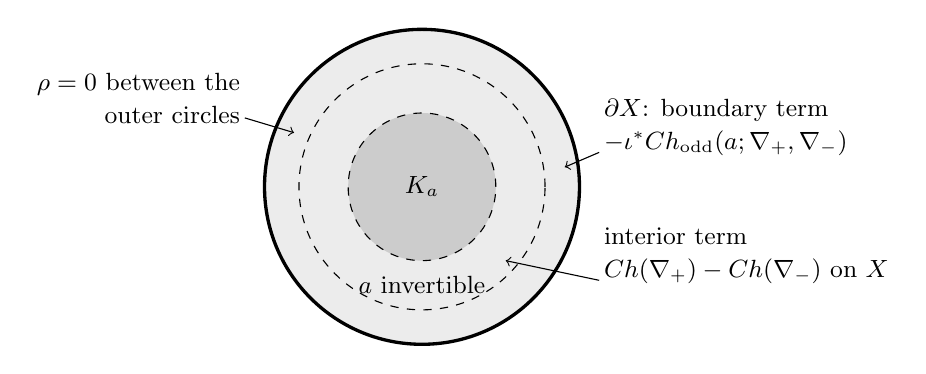
\begin{tikzpicture}[scale=1.25]
  \fill[gray!15] (0,0) circle (1.6);
  \fill[gray!40] (0,0) circle (0.75);
  \draw[very thick] (0,0) circle (1.6);
  \draw[dashed] (0,0) circle (0.75);
  \draw[dashed] (0,0) circle (1.25);
  \node at (0,0) {\small$K_a$};
  \node at (0,-1.0) {\small$a$ invertible};
  \node[right,align=left] at (1.75,0.6) {\small$\partial X$: boundary term\\
    \small$-\iota^*\Chodd(a;\nabla_+,\nabla_-)$};
  \node[right,align=left] at (1.75,-0.7) {\small interior term\\
    \small$\Ch(\nabla_+)-\Ch(\nabla_-)$ on $X$};
  \draw[->] (1.8,0.35)--(1.45,0.2);
  \draw[->] (1.8,-0.95)--(0.85,-0.75);
  \node[left,align=right] at (-1.75,0.9) {\small$\rho=0$ between the\\
    \small outer circles};
  \draw[->] (-1.8,0.7)--(-1.3,0.55);
\end{tikzpicture}
\caption[The relative Chern character]{A fibre of the radially compactified
cotangent bundle $X$. The symbol $a$ fails to be invertible only in the compact set
$K_a$. The representative $\lambda_\rho$ of \eqref{families:eq:lambda-rho} is a
compactly supported form, obtained by bending the connection on $E_+$ into
$a^{-1}\nabla_-a$ before reaching $\partial X$. The Fedosov-type formula
(\cref{families:thm:fedosov}) instead keeps the two given connections up to the
boundary and pays for it with an odd Chern--Simons form of the symbol on
$\partial X=S^*(M/B)$.}
\label{families:fig:relative}
\end{figure}

\begin{discussion}
  The two representatives in \cref{families:fig:relative} correspond to the two
  descriptions of $H^*_{\mathrm c}(\operatorname{int}X)=H^*(X,\partial X)$: a
  compactly supported closed form, or a closed form on $X$ together with a
  primitive of its restriction to $\partial X$. For the symbol of an elliptic
  family the second is more natural, because the symbol is given at infinity,
  that is on $\partial X$, and the boundary term is then built from
  $a^{-1}\nabla a$ alone. When the bundles are trivial with trivial connections,
  the interior term vanishes and the whole class is carried by the odd Chern
  form of the symbol on the cosphere bundle; this is the form of the index formula
  used in \cref{ch:eta}.
\end{discussion}

\begin{remark}\label{families:rem:conormal}
  The formula can be obtained by letting $\rho$ tend to the characteristic
  function of $X$. Let $x$ be a boundary defining function and
  $\rho=\chi(x/\epsilon)$ with $\chi\in\CI(\R)$, $\chi=0$ on $(-\infty,\frac12]$,
  $\chi=1$ on $[1,\infty)$. From \eqref{families:eq:nabla-rho},
  \begin{equation*}
    \omega_{\nabla^\rho}=\Omega(1-\rho)-d\rho\wedge\gamma,
  \end{equation*}
  and since $(d\rho)^2=0$, $\tr e^{c\omega_{\nabla^\rho}}=\tr e^{c\Omega(1-\rho)}
  -c\,d\rho\wedge\tr(\gamma e^{c\Omega(1-\rho)})$. As $\epsilon\to0$ the first
  term tends to $\tr e^{c\omega_+}$ boundedly almost everywhere. In the second,
  $d\rho=\epsilon^{-1}\chi'(x/\epsilon)dx$; replacing the coefficients by
  their boundary values (with an error that tends to zero) and substituting
  $s=1-\chi(x/\epsilon)$ shows that it converges, as a current, to
  $\delta(x)dx\wedge\nu$ with $\nu=-c\,\iota^*\int_0^1\tr(\gamma e^{c\Omega(s)})ds$
  (here $\int\epsilon^{-1}\chi'(x/\epsilon)f(1-\chi(x/\epsilon))\,dx=\int_0^1f(s)\,ds$).
  To make sense of currents supported at the boundary we use the following
  convention: $x$ increases into $X$, forms on $X$ and on $\partial X$ are
  extended by zero across $\partial X$ to a collar $(-1,1)_x\times\partial X$
  in a slightly larger manifold (or to the double of $X$), and $\nu$ is
  extended to the collar independently of $x$. The limit is then the
  ``conormal'' current
  \begin{equation*}
    1_{x>0}\,\mu+\delta(x)dx\wedge\nu,\qquad\mu=\tr e^{c\omega_+}-\tr e^{c\omega_-},
  \end{equation*}
  with $(\mu,\nu)$ exactly the pair of \cref{families:thm:fedosov}. Since
  $d(1_{x>0})=\delta(x)dx$ and $d(\delta(x)dx\wedge\nu)=-\delta(x)dx\wedge d\nu$,
  \begin{equation*}
    d\bigl(1_{x>0}\,\mu+\delta(x)dx\wedge\nu\bigr)=1_{x>0}\,d\mu
    +\delta(x)dx\wedge(\iota^*\mu-d\nu)
  \end{equation*}
  (only the tangential part $\iota^*\mu$ survives next to $\delta(x)dx$). So the
  current is closed exactly when $d\mu=0$ and $\iota^*\mu=d\nu$, which is the
  closedness of the pair in \cref{families:thm:fedosov}; and pairing it with a
  closed form $\varphi$ on an oriented $X$ (extended smoothly into the collar) gives \eqref{families:eq:rel-pairing},
  since $\int_X\delta(x)dx\wedge\beta=-\int_{\partial X}\iota^*\beta$ for the
  boundary orientation (the outward normal is $-\partial_x$). The proof given above avoids distributions.
  Note the analogy with \cref{families:prop:toeplitz-chern}, where the index
  class is also given by an integral of the odd forms of the symbol over a
  boundary circle.
\end{remark}

For an elliptic family $A\in\Psido0(M/B;E_+,E_-)$ we apply this with $X$ the
radial compactification of $T^*(M/B)$ (a ball bundle), $\partial X=S^*(M/B)$,
the lifted bundles with pulled-back connections, and $a=\sigma_0(A)$
homogeneous. This defines
\begin{equation*}
  \Ch(\sigma_0(A))\in H^{\mathrm{ev}}_{\mathrm c}(T^*(M/B);\C),
\end{equation*}
represented by the pair of \cref{families:thm:fedosov}, whose second entry
lives on $S^*(M/B)$ and is built from $\sigma_0(A)^{-1}\nabla\sigma_0(A)$.

\subsection{The odd Chern character as a suspension}
The constants $c_k$ in \eqref{families:eq:Chodd} were fixed by the Toeplitz index. They are
also forced by the even Chern character, through the clutching construction: the odd
Chern character of $g$ is the fibre integral of the Chern character of the compactly
supported class on $\R\times X$ obtained by clutching with $g$. We use the
integral form of $\Chodd$.

\begin{lemma}\label{families:lem:Chodd-integral}
  For $g\in\CI(X;\GL(N,\C))$, with $\theta=g^{-1}dg$ and $c=i/2\pi$,
  \begin{equation*}
    \Chodd(g)=c\int_0^1\tr\Bigl(\theta\,\exp\bigl(c\,s(s-1)\,\theta^2\bigr)\Bigr)ds .
  \end{equation*}
\end{lemma}
\begin{proof}
  The term of degree $2k+1$ on the right is
  $\frac{c^{k+1}}{k!}\int_0^1(s^2-s)^kds\,\tr(\theta^{2k+1})$, and
  $\int_0^1(s^2-s)^kds=(-1)^k\int_0^1s^k(1-s)^kds=(-1)^k\frac{(k!)^2}{(2k+1)!}$. So the
  coefficient is $c(-c)^k\frac{k!}{(2k+1)!}=\frac{i}{2\pi}\bigl(\frac{-i}{2\pi}\bigr)^k\frac{k!}{(2k+1)!}=c_k$.
\end{proof}

For compact $X$ and $g\in\CI(X;\GL(N,\C))$ let
\begin{equation*}
  \operatorname{clu}[g]=\bigl[(\C^N,\C^N,\tilde g)\bigr]\in\Kc(\R\times X),\qquad
  \tilde g(t,x)=\Id\ (t\le-1),\quad\tilde g(t,x)=g(x)\ (t\ge1),
\end{equation*}
the clutching isomorphism $K^{-1}(X)\cong\Kc(\R\times X)$ of \cref{ch:bott}. We regard
$\R\times X$ as the interior of a compact manifold with boundary by compactifying $\R$ to
a closed interval, so that \cref{families:prop:relative-chern} applies, and for a
compactly supported form $\mu=dt\wedge\mu_1+\mu_2$ on $\R\times X$ ($\mu_1$, $\mu_2$
without $dt$) set $\int_\R\mu=\int_{\R}\mu_1\,dt$. As for $\int_\Sphere$ in
\cref{families:sec:toeplitz}, this anticommutes with $d$, $\int_\R d\mu=-d\int_\R\mu$,
because the $dt$-component of $d\mu$ is $dt\wedge(-d_X\mu_1+\partial_t\mu_2)$ and
$\partial_t\mu_2$ integrates to zero by compact support; so it maps closed forms to
closed forms and exact forms to exact forms, and induces a map in cohomology.

\begin{proposition}\label{families:prop:Chodd-clutching}
  For compact $X$ and $g\in\CI(X;\GL(N,\C))$,
  \begin{equation*}
    \int_\R\Ch\bigl(\operatorname{clu}[g]\bigr)=\Chodd(g)\in\Hodd(X;\C).
  \end{equation*}
  In fact, for the trivial connections and a suitable cut-off, the representative
  $\lambda_\rho$ of \eqref{families:eq:lambda-rho} satisfies $\int_\R\lambda_\rho=\Chodd(g)$ as
  forms.
\end{proposition}
\begin{proof}
  Take $\nabla_\pm=d$ on $E_\pm=\C^N$. Where $\tilde g$ is invertible,
  $\gamma=\tilde g^{-1}d\tilde g$ is $0$ for $t\le-1$ and $\theta=g^{-1}dg$ for $t\ge1$. Choose
  $\chi\in\CI(\R)$ with $\chi=0$ on $(-\infty,1]$, $\chi=1$ on $[2,\infty)$, and $\rho$ with
  $\rho=1-\chi$ on $[0,\infty)$, $\rho=1$ on $[-1,0]$ and $\rho=0$ near $-\infty$; since
  $\gamma=0$ for $t\le-1$, \eqref{families:eq:nabla-rho} is $\nabla^\rho=d+\chi(t)\theta$. Its
  curvature is, using $d\theta=-\theta^2$,
  \begin{equation*}
    \omega=d(\chi\theta)+\chi^2\theta^2=d\chi\wedge\theta+(\chi^2-\chi)\theta^2 .
  \end{equation*}
  The two terms commute, because both are built from powers of the same
  matrix-valued $1$-form $\theta$ with scalar coefficients: both products equal
  $(\chi^2-\chi)\,d\chi\wedge\theta^3$ (moving the scalar $1$-form $d\chi$ past
  $\theta^2$ produces no sign). Moreover $(d\chi\wedge\theta)^2=0$, so
  $\tr e^{c\omega}=\tr e^{c(\chi^2-\chi)\theta^2}+c\,d\chi\wedge\tr\bigl(\theta e^{c(\chi^2-\chi)\theta^2}\bigr)$.
  Hence $\lambda_\rho=\tr e^{c\omega}-N$ is supported in $1\le t\le2$, and
  \begin{equation*}
    \int_\R\lambda_\rho=c\int_\R\chi'(t)\tr\bigl(\theta e^{c(\chi^2-\chi)\theta^2}\bigr)dt
    =c\int_0^1\tr\bigl(\theta e^{c(s^2-s)\theta^2}\bigr)ds=\Chodd(g)
  \end{equation*}
  by the substitution $s=\chi(t)$ and \cref{families:lem:Chodd-integral}.
\end{proof}

\begin{remark}\label{families:rem:Chodd-fedosov}
  More generally, for a bundle isomorphism $a\colon F\to F'$ and connections on $F$, $F'$, the
  form
  \begin{gather*}
    \Chodd(a;\nabla_F,\nabla_{F'})=c\int_0^1\tr\bigl(\gamma\,e^{c\Omega(s)}\bigr)ds,\\
    \gamma=a^{-1}\nabla a,\qquad\Omega(s)=(1-s)\omega_F+s\,a^{-1}\omega_{F'}a+s(s-1)\gamma^2,
  \end{gather*}
  reduces to \cref{families:lem:Chodd-integral} for trivial bundles and connections. It is
  the Chern--Simons form of the path $\nabla_F+s\gamma$ from $\nabla_F$ to $a^{-1}\nabla_{F'}a$, so
  $d\Chodd(a;\nabla_F,\nabla_{F'})=\Ch(\nabla_{F'})-\Ch(\nabla_F)$, and
  \cref{families:thm:fedosov} says that the relative Chern character of $(E_+,E_-,a)$ is
  represented by the pair $\bigl(\Ch(\nabla_+)-\Ch(\nabla_-),-\iota^*\Chodd(a;\nabla_+,\nabla_-)\bigr)$:
  the boundary term is the odd Chern character of the symbol. The proof of
  \cref{families:prop:Chodd-clutching} is the special case in which the second entry is moved
  into the interior.
\end{remark}

\section{The cohomological form of the index theorem}\label{families:sec:cohomology}

Orient the fibres $T^*_{b}(Z)$ of $\pi:T^*(M/B)\to B$, where $\pi$ is the
composite of the bundle projection and $\phi$, by
$dz_1\wedge d\zeta_1\wedge\dots\wedge dz_n\wedge d\zeta_n$ in canonical
coordinates ($z$ coordinates on the fibre $Z_b$, $\zeta$ the dual
coordinates). This is the $n$-th power of the canonical symplectic form (up to
a universal sign), so it is well defined even if $Z$ is not orientable.
Integration over the fibres is then a map
$\pi_*:H^*_{\mathrm c}(T^*(M/B))\to H^{*-2n}(B)$. Let $\Td$ denote the Todd
class, the multiplicative characteristic class with $\Td(L)=c_1(L)/(1-e^{-c_1(L)})$
for a line bundle $L$.

\begin{theorem}[Atiyah--Singer, cohomological form]\label{families:thm:AS-H}
  For every $x\in\Kc(T^*(M/B))$, with $n$ the dimension of the fibres of $\phi$,
  \begin{equation*}
    \Ch\bigl(\inda(x)\bigr)=(-1)^n\pi_*\bigl(\Ch(x)\wedge\pi_0^*\Td(T(M/B)
    \otimes\C)\bigr)\in\Hev(B;\C),
  \end{equation*}
  $\pi_0:T^*(M/B)\to M$ the projection. In particular, for an elliptic family
  $A$, $\Ch(\ind A)=(-1)^n\int_{T^*(M/B)/B}\Ch(\sigma_0(A))\Td(T(M/B)\otimes\C)$.
\end{theorem}

This is \cite{Atiyah-Singer-IV}, Theorem~5.1, and we do not give a
self-contained proof of it. Since the sign depends on the
orientation convention, it is often absorbed into it, as in the form
$\Ch(\ind A)=\int\Td\cdot\Ch(\sigma(A))$. We explain how the theorem follows
from \cref{families:thm:AS-K}; the two topological inputs used, the
multiplicativity \ref{families:C1} for compactly supported classes and the
Riemann--Roch identity \ref{families:C4} for non-trivial $\mathcal V$, are
imported (see the Notes); everything else in the derivation is proved in
this chapter.

\begin{discussion}
  Where does the Todd class come from? Apply $\Ch$ to each arrow of
  \cref{families:fig:roadmap}. The extension $j_*\Theta_*$ is harmless, and
  $\beta_N^{-1}$ becomes integration over $\R^{2N}$ up to a sign. The Thom map $\tau$
  multiplies by $\lambda_{\mathcal V}$, and in cohomology this becomes ``integrate
  over the normal directions'' only up to a correction factor: the fibre integral of
  $\Ch(\lambda_{\mathcal V})$ is not $\pm1$ but $\pm\Td(\mathcal V\otimes\C)^{-1}$.
  Since $\mathcal V$ is a complement of $T(M/B)$, this correction is
  $\Td(T(M/B)\otimes\C)$. In other words, the Todd class measures the failure of
  the Chern character to commute with the Thom isomorphism
  (\cref{families:rem:todd-thom}).
\end{discussion}

\begin{proof}[Derivation from \cref{families:thm:AS-K}]
  We use the following properties of the Chern character of
  \cref{families:prop:relative-chern}.
  \begin{enumerate}[label=(C\arabic*)]
  \item\label{families:C1} $\Ch$ is multiplicative for the products of
    \cref{families:def:product}: $\Ch(x_1\cdot x_2)=\Ch(x_1)\wedge\Ch(x_2)$.
    (This is standard; on a compact space it is \cref{families:prop:chern}(iii),
    and the compactly supported case follows by passing to one-point
    compactifications.)
  \item\label{families:C2} $\Ch$ commutes with extensions $j_*$ for open
    embeddings (extension of compactly supported forms by zero) and with
    pull-backs, since the forms $\lambda_\rho$ are compactly supported and
    natural.
  \item\label{families:C3} $\int_{T^*I}\Ch(b_1)=-1$ for the orientation
    $d\theta\wedge d\xi$ (\cref{families:ex:bott-chern}). Hence by
    \ref{families:C1}, \ref{families:C2},
    $\Ch(\beta_N^{-1}z)=(-1)^N\pi_*\Ch(z)$ for $z\in\Kc(T^*I^N\times B)$, with
    the orientation above on $T^*I^N$.
  \item\label{families:C4} For a real vector bundle $\mathcal V$ of rank $k$
    over $M$, integration over the fibres of $T^*(\mathcal V/M)\cong\mathcal
    V\otimes\C$ gives
    $\varpi_*\Ch(\lambda_{\mathcal V})=(-1)^k\Td(\mathcal V\otimes\C)^{-1}$.
    For trivial $\mathcal V$ this is \ref{families:C3} with $B=M$ and
    \cref{families:rem:bott-generator}; in general it is the classical
    Riemann--Roch computation of Atiyah and Hirzebruch, in the form proved in
    \S2 of Atiyah--Singer~III (see the Notes), which we import.
  \item\label{families:C5} $\Td$ is multiplicative and
    $T(M/B)\oplus\mathcal V$ is trivial, so $\Td(\mathcal V\otimes\C)^{-1}=
    \Td(T(M/B)\otimes\C)$.
  \end{enumerate}
  Then, with $x\in\Kc(T^*(M/B))$ and the orientations multiplying as they
  should (all of them are products of oriented two-planes),
  \begin{align*}
    \Ch(\inda x)&=\Ch\bigl(\beta_N^{-1}j_*\Theta_*\tau(x)\bigr)
    =(-1)^N\pi_*\Ch(\lambda_{\mathcal V}\cdot\varpi^*x)\\
    &=(-1)^N\pi_*\bigl(\varpi_*\Ch(\lambda_{\mathcal V})\wedge\Ch(x)\bigr)
    =(-1)^{N+k}\pi_*\bigl(\Td(T(M/B)\otimes\C)\wedge\Ch(x)\bigr),
  \end{align*}
  and $(-1)^{N+k}=(-1)^n$ since $N=n+k$.
\end{proof}

\begin{remark}\label{families:rem:todd-structure}
  Even without (C4) the derivation shows that $\Ch(\inda x)=\pi_*(\Ch(x)\wedge
  \pi_0^*\mathcal T)$ for a class $\mathcal T\in\Hev(M;\C)$ which depends only
  on the fibration (through its normal bundle), not on $x$. The content of (C4)
  is the identification of $\mathcal T$ with $(-1)^n\Td(T(M/B)\otimes\C)$.
  For $B$ a point and $n=1$, $M=\Sphere$, the theorem reduces to
  $\ind(P_1)=1=-\int_{T^*\Sphere}\Ch(\sigma_0(P_1))$, which is
  \cref{families:ex:bott-chern}.
\end{remark}

\begin{remark}[The Todd class and the Thom isomorphism]\label{families:rem:todd-thom}
  The class $\mathcal T$ can be described through the Thom isomorphism of \cref{ch:bott}.
  Let $V\to M$ be a Hermitian complex vector bundle of rank $n$, $\varpi\colon V\to M$, with
  Bott class $\beta_V\in\Kc(V)$ (for $V=\mathcal V\otimes\C$ this is $\lambda_{\mathcal V}$), and orient
  the fibres as complex vector spaces. By \cref{ch:bott}, $x\mapsto\beta_V\cdot\varpi^*x$ is an
  isomorphism $K^0(M)\to\Kc(V)$, with inverse $\operatorname{Thom}_V$. By \ref{families:C1}
  and the projection formula $\varpi_*(\varpi^*\alpha\wedge\mu)=\alpha\wedge\varpi_*\mu$ for even $\alpha$,
  \begin{equation*}
    \varpi_*\Ch(\beta_V\cdot\varpi^*x)=\Ch(x)\wedge\varpi_*\Ch(\beta_V).
  \end{equation*}
  Restricted to a point, $\beta_V$ is the $n$-fold product of the class $b_1=\lambda_\R$ of
  \cref{families:rem:bott-generator}, so by \ref{families:C1}, \ref{families:C3} the degree zero part of
  $\varpi_*\Ch(\beta_V)$ is $(-1)^n$, and
  $\mathcal T(V)=(-1)^n\bigl(\varpi_*\Ch(\beta_V)\bigr)^{-1}\in\Hev(M;\C)$ is defined. Thus
  \begin{equation*}
    \Ch\bigl(\operatorname{Thom}_V(y)\bigr)=(-1)^n\varpi_*\Ch(y)\wedge\mathcal T(V),\qquad y\in\Kc(V).
  \end{equation*}
  Since $\beta_{V\oplus W}=\beta_V\cdot\beta_W$ and $\beta$ is natural, $\mathcal T$ is a multiplicative
  characteristic class with $\mathcal T(\C^n)=1$; if $V\oplus W$ is trivial of rank $m$, then
  $\mathcal T(V)=(-1)^{\operatorname{rank}W}\varpi_*\Ch(\beta_W)$, which is the definition of the Todd class
  as the fibre integral of the Chern character of the Bott element of a complement used in
  the source. The identification of $\mathcal T(\mathcal V\otimes\C)$ with
  $\Td(\mathcal V\otimes\C)$ is \ref{families:C4}, which is imported and not
  proved here; the only parts of this remark proved in the text are the
  projection formula and the normalization of the degree zero part (from
  \ref{families:C3}), while the multiplicativity of $\mathcal T$ uses
  \ref{families:C1}, also imported, and the Thom isomorphism of
  \cref{ch:bott}. The orientation is the complex one on the fibres of $V$,
  which for $V=\mathcal V\otimes\C$ is the orientation by products of oriented
  two-planes $dv_j\wedge d\eta_j$ used in \ref{families:C4}.
\end{remark}

\section{Exercises}

\begin{exercise}\label{families:ex:ext-product}
  Show directly that the exterior product of \cref{families:def:product} is
  well defined on $\Kc$-classes and bilinear, and that $x\boxtimes y$
  corresponds to $y\boxtimes x$ under the flip $X_1\times X_2\cong X_2\times
  X_1$. (For the latter, find a homotopy between $a_1\#a_2$ and the
  conjugate of $a_2\#a_1$ by the obvious bundle isomorphisms.)
\end{exercise}

\begin{exercise}\label{families:ex:CP1}
  Complete \cref{families:ex:grassmann}: show that for the tautological line
  bundle over $\C P^1$, $\frac{i}{2\pi}\tr(\pi(d\pi)^2)=-\frac{1}{\pi}(1+\abs
  w^2)^{-2}dx\wedge dy$ in the affine coordinate $w=x+iy$, so that its integral
  is $-1$.
\end{exercise}

\begin{exercise}\label{families:ex:bott-chern}
  Let $X\subset T^*I$ be a large square $[\epsilon,2\pi-\epsilon]\times[-R,R]$
  in the coordinates $(\theta,\xi)$, oriented by $d\theta\wedge d\xi$, and
  represent $b_1$ by the trivial bundles with the trivial connection and the
  symbol of \eqref{families:eq:P1} modified as in the definition of $b_1$.
  Use \cref{families:thm:fedosov} with $\varphi=1$ to show that
  $\int_{T^*I}\Ch(b_1)=\frac{i}{2\pi}\int_{\partial X}a^{-1}da=-1$.
\end{exercise}

\begin{exercise}\label{families:ex:odd-product}
  Show that for maps $a,a':X\to\GL(N,\C)$ the forms $\Chodd(aa')$ and
  $\Chodd(a)+\Chodd(a')$ differ by an exact form. (Use the homotopy
  $\bigl(\begin{smallmatrix}a&0\\0&1\end{smallmatrix}\bigr)R_t
  \bigl(\begin{smallmatrix}a'&0\\0&1\end{smallmatrix}\bigr)R_t^{-1}$ with
  $R_t$ a rotation from $\Id$ to $\bigl(\begin{smallmatrix}0&1\\-1&0
  \end{smallmatrix}\bigr)$, and \eqref{families:eq:odd-transgression}.)
\end{exercise}

\begin{exercise}\label{families:ex:pullback-index}
  Prove the base change property \cref{families:rem:stab-remarks}(d) in detail,
  and deduce that if $\inda(b)=1$ in $K^0(M)$ for $b\in\Kc(T^*(\tilde M/M))$
  then the restriction of $b$ to the fibre over any $m\in M$ has numerical
  index $1$.
\end{exercise}

\begin{exercise}\label{families:ex:winding}
  Show that $\Kc(\R^2)\to\Z$, taking the class of a triple
  $(\C^r,\C^r,a)$ with $a$ invertible outside a disc to the winding number of
  $\det a$ on a large circle, is well defined, and that it maps $b_1$ to $1$.
  Deduce from \cref{families:prop:normalization} with $N=1$ and $B$ a point
  that the index of a symbol in $\Kc(T^*I)$, extended to the circle, equals
  this winding number.
\end{exercise}

\section*{Notes}
This chapter follows Lectures 19--21 of the 2005 course, with several
changes. The proofs of multiplicativity and excision were completed: the
invertibility of the symbols along the deformation is now deduced from the
single identity of \cref{families:lem:clifford}; the families index of
product-type families and the comparison of the stabilization by sections with
the construction of \cref{ch:product} (left to the addenda in the original)
are in \cref{families:lem:stabilization}; the hypothesis of a trivialized null
line bundle is reduced to $\inda(b)=1$ in \cref{families:lem:normalize-P}.
The normalization on the trivial fibration is proved via multiplicativity on
the torus. In the original the curvature of the Grassmann connection carries
a sign error, which propagated to the constants in the formula for the Chern
character of a Toeplitz index; the corrected constants are in
\eqref{families:eq:Chodd} (we checked the case $k=1$ also numerically).
The original section on the Bott element was empty; here its role is played
by $P_1$, the normalization proposition and the imported statement
\ref{families:TH}.

The families index theorem is due to Atiyah and Singer
\cite{Atiyah-Singer-IV}; the K-theoretic method of proof, by embedding,
excision and multiplicativity, goes back to M.~F. Atiyah and I.~M. Singer,
\emph{The index of elliptic operators~I}, Ann. of Math. \textbf{87} (1968),
484--530, where the equivariant index of the Bott operator needed for
\ref{families:TH} is computed. For K-theory, products, the Thom isomorphism
and Bott periodicity see \cite{Atiyah-K}. The Riemann--Roch identity
\ref{families:C4} and the theorem that the Chern character is a rational
isomorphism are due to M.~F. Atiyah and F. Hirzebruch, \emph{Vector bundles
and homogeneous spaces}, Proc. Sympos. Pure Math. \textbf{3} (1961), 7--38,
and M.~F. Atiyah and F. Hirzebruch, \emph{Riemann--Roch theorems for
differentiable manifolds}, Bull. Amer. Math. Soc. \textbf{65} (1959),
276--281; the form \ref{families:C4} of the identity, for the Thom class of
$\mathcal V\otimes\C$ with the orientation used here, is derived in \S2 of
M.~F. Atiyah and I.~M. Singer, \emph{The index of elliptic operators~III},
Ann. of Math. \textbf{87} (1968), 546--604, where the cohomological formula is
deduced from the K-theoretic one in the same way as above. The
multiplicativity \ref{families:C1} of the Chern character on compactly
supported K-theory is standard (\cite{Atiyah-K} and the same \S2). The
existence of the embedding in \cref{families:lem:embedding} is Whitney's
theorem (H. Whitney, \emph{Differentiable manifolds}, Ann. of Math.
\textbf{37} (1936), 645--680; see e.g. J.~M. Lee, \emph{Introduction to smooth
manifolds}, 2nd ed., Springer, New York, 2013, Theorem~6.15).
The explicit formula of \cref{families:thm:fedosov} is of the type used by
B.~V. Fedosov in his work on index formulas.

The material on Chern forms, the odd Chern character, and the Todd class in the K-theory
chapter of the 2008 revision of the lectures (\emph{From microlocal to global analysis})
has been merged here. There the odd Chern character is derived from a connection on the
bundle over $\Sphere\times X$ clutched by $g$, which yields the integral formula of
\cref{families:lem:Chodd-integral}; the source leaves its constants open (and, with an
unnormalized even Chern character $\tr e^{\omega}$, warns of possible sign errors). With the
normalization $\tr e^{i\omega/2\pi}$ the clutching computation
(\cref{families:prop:Chodd-clutching}) reproduces exactly the constants $c_k$ of
\eqref{families:eq:Chodd} that were fixed by the Toeplitz index, a non-trivial consistency
check, and the source's general formula for an isomorphism of bundles with connections is the
boundary term of \cref{families:thm:fedosov} (\cref{families:rem:Chodd-fedosov}). The source
states the Chern character of the isotropic index as $-\frac1{2\pi i}\int\Chodd$ for
unnormalized forms and its own orientation of the circle; in our conventions it is
\cref{families:rem:iso-chern}. The source defines the Todd class of $E$ as the fibre integral
of the Chern character of the Bott element of a complement; \cref{families:rem:todd-thom}
shows how this follows from the Thom isomorphism, with the signs made explicit.
